\documentclass[11pt]{article}
\usepackage[utf8]{inputenc}
\usepackage[T1]{fontenc}
\usepackage[turkish]{babel}
\usepackage[margin=1in]{geometry}

\usepackage{amsmath,amssymb}
\usepackage{booktabs}
\usepackage{graphicx}
\usepackage{subcaption}
\usepackage{multirow}
\usepackage{array}
\usepackage{xcolor}
\usepackage{tikz}
\usetikzlibrary{positioning,arrows.meta,fit,backgrounds,calc,shadows.blur}
\usepackage{algorithm}
\usepackage{algpseudocode}
\usepackage{hyperref}
\hypersetup{colorlinks=true, linkcolor=blue, citecolor=blue, urlcolor=blue}

\graphicspath{{figures/}{./}}

\setlength{\parindent}{12pt}
\setlength{\parskip}{0.4\baselineskip}

% Renkler (mimari diyagram için)
\definecolor{frozen}{RGB}{210,214,220}
\definecolor{trainable}{RGB}{255,196,120}
\definecolor{datablk}{RGB}{180,215,245}

\title{\textbf{Göğüs Röntgeni Üretimi için Metin-Koşullu Difüzyon
Modellerinin Kaynak-Verimli Alan Uyarlaması: Tam İnce Ayar ile
Parametre-Verimli Uyarlamanın Sistematik Karşılaştırması}\\[6pt]
\large Resource-Efficient Domain Adaptation of Text-Conditioned Diffusion
Models for Synthetic Chest X-ray Generation}

\author{Ömer Atılım KOCA -- 6041013 \qquad Emre TURAN -- 6041014\\[2pt]
İzmir Bakırçay Üniversitesi, Bilgisayar Mühendisliği Doktora Programı\\
BIL 941 -- Derin Üretken Modellerin Uygulamaları}
\date{\today}

\begin{document}
% Türkçe babel '=' karakterini aktif shorthand yapar; tikz/includegraphics/
% algoritma gibi key-value ortamları bozulmasın diye kapatıyoruz.
\shorthandoff{=}
\maketitle

\begin{abstract}
\noindent
Etiketli ve yüksek kaliteli tıbbi görüntü veri kümelerinin sınırlı erişilebilirliği,
derin öğrenme modellerinin klinik ortamlardaki genelleme başarımını kısıtlayan
önemli etkenlerden biridir. Metin-koşullu latent difüzyon modelleri, radyolojik
raporlar gibi serbest metin açıklamalarıyla yönlendirilebilen sentetik görüntüler
üreterek bu kısıtı azaltma potansiyeli sunmaktadır. Bununla birlikte, mevcut
yaklaşımların önemli bir bölümü yüksek hesaplama kaynaklarına ihtiyaç duymakta
ve bu durum yöntemlerin erişilebilir donanımlarda uygulanabilirliğini
sınırlamaktadır.

Bu çalışmada, Stable Diffusion v1.4 modelinin MIMIC-CXR veri kümesi kullanılarak
göğüs röntgeni alanına uyarlanması, tek-GPU kısıtı altında incelenmiştir. Tam
ince ayar yaklaşımı, düşük-rank parametre-verimli uyarlama yöntemi olan LoRA ile
aynı eğitim bütçesi altında karşılaştırılmıştır. Ayrıca üretim çözünürlüğü,
rank-kararlı LoRA ölçeklemesi ve patoloji-ödül tabanlı ek kayıp bileşeninin
etkileri kontrollü ablasyon deneyleriyle değerlendirilmiştir.

Deneysel sonuçlar, incelenen kaynak-kısıtlı koşullarda LoRA tabanlı uyarlamanın
tam ince ayara kıyasla daha düşük bellek kullanımı, daha kısa eğitim süresi ve
daha iyi alan-içi dağılım uyumu sağladığını göstermektedir. Özellikle LoRA
yaklaşımı, eğitilebilir parametrelerin yalnızca küçük bir bölümünü kullanmasına
rağmen FID$_{\text{XRV}}$ metriğinde tam ince ayardan daha düşük değer elde
etmiştir. Buna karşılık, sabit eğitim bütçesi altında çözünürlüğün veya
eğitilebilir rank değerinin artırılması tutarlı bir kalite artışı sağlamamış;
patoloji-ödül bileşeni ise üretim sadakatini olumsuz etkilemiştir.

Bu bulgular, metin-koşullu tıbbi görüntü üretiminde model kapasitesinden çok,
sınırlı hesaplama bütçesi altında kapasitenin nasıl tahsis edildiğinin ve
optimizasyon koşullarının belirleyici olabileceğine işaret etmektedir.
Çalışma, erişilebilir donanımlarda tıbbi difüzyon modeli uyarlaması için
LoRA tabanlı yaklaşımların pratik değerini ortaya koymakta ve zaman-adımına
duyarlı düşük-rank uyarlama stratejileri için gelecek araştırmalara zemin
hazırlamaktadır.

\smallskip
\noindent\textbf{Anahtar kelimeler:} Latent difüzyon modelleri, göğüs röntgeni,
metin-koşullu görüntü üretimi, parametre-verimli ince ayar, LoRA, tıbbi görüntü
sentezi.
\end{abstract}
% ============================================================================
\section{Giriş}
% ============================================================================

Derin öğrenme tabanlı görüntü çözümleme yöntemleri, yeterli miktarda, dengeli
dağılıma sahip ve güvenilir biçimde etiketlenmiş veri kümeleri üzerinde
eğitildiklerinde yüksek başarım gösterebilmektedir. Bununla birlikte, tıbbi
görüntüleme alanında bu koşullar çoğu zaman sınırlı biçimde sağlanabilmektedir.
Uzman anotasyonunun maliyetli ve zaman alıcı olması, hasta mahremiyetine ilişkin
kısıtlar, kurumlar arası veri paylaşımındaki güçlükler ve nadir patolojilerin
veri kümelerinde az temsil edilmesi, klinik uygulamalara yönelik modellerin
genelleme başarımını olumsuz etkileyen temel faktörler arasında yer almaktadır.
Bu nedenle, tıbbi görüntüleme alanında veri yetersizliğini azaltabilecek,
alan-tutarlı ve kontrollü sentetik örnekler üretebilecek yöntemlere yönelik
ilgi giderek artmaktadır~\cite{roentgen,mimic}.

Sentetik veri üretimi, özellikle veri paylaşımının kısıtlı olduğu veya belirli
patolojilerin sınırlı sayıda örnekle temsil edildiği klinik senaryolarda
potansiyel bir çözüm olarak değerlendirilmektedir. Bu bağlamda üretken modeller,
gerçek hasta verisini doğrudan çoğaltmadan, hedef alanın görsel ve semantik
özelliklerini yansıtan yeni örnekler üretmeyi amaçlar. Geleneksel olarak tıbbi
görüntü sentezinde üretken çekişmeli ağlar (GAN) yaygın biçimde kullanılmış
olsa da, eğitim kararsızlığı, mod çökmesi ve koşullandırma kabiliyetinin sınırlı
kalması gibi sorunlar bu yaklaşımların kullanımını kısıtlayabilmektedir. Son
yıllarda difüzyon tabanlı üretken modeller, daha kararlı eğitim süreçleri ve
yüksek görsel kalite üretme kapasiteleri nedeniyle tıbbi görüntü sentezinde
dikkat çekici bir alternatif haline gelmiştir~\cite{ddpm,medfusion}.

Difüzyon modelleri, veriye kademeli olarak gürültü ekleyen bir ileri süreç ve
bu süreci tersine çevirmeyi öğrenen bir gürültü giderme süreci üzerine kuruludur.
Ancak yüksek çözünürlüklü görüntüler üzerinde doğrudan piksel uzayında çalışmak
yüksek hesaplama maliyeti gerektirdiğinden, latent difüzyon modelleri (LDM)
bu süreci daha düşük boyutlu bir gizil uzayda gerçekleştirerek önemli bir
verimlilik avantajı sağlamaktadır~\cite{ldm}. Bu yaklaşımın metin koşullandırma
mekanizmalarıyla birleştirilmesi, Stable Diffusion gibi büyük ölçekli
metinden-görüntüye üretim modellerinin ortaya çıkmasına olanak sağlamıştır.
Söz konusu modeller, doğal görüntü--metin çiftleri üzerinde önceden
eğitildiklerinden, uygun ince ayar stratejileriyle farklı alanlara
uyarlanabilen güçlü temel modeller olarak değerlendirilmektedir.

Stable Diffusion modelinin tıbbi görüntüleme alanına uyarlanmasına yönelik
önemli çalışmalardan biri RoentGen'dir~\cite{roentgen}. RoentGen, MIMIC-CXR
veri kümesini kullanarak Stable Diffusion modelini göğüs röntgeni üretimi için
ince ayarlamış ve radyolojik metin istemleriyle koşullandırılmış sentetik CXR
görüntülerinin üretilebileceğini göstermiştir. Bu çalışma, metin-koşullu
difüzyon modellerinin tıbbi görüntü sentezi ve veri artırma bağlamındaki
potansiyelini ortaya koyması bakımından önemli bir referans niteliğindedir.
Bununla birlikte, RoentGen'in eğitim süreci yüksek hesaplama kaynaklarına
dayanmaktadır; model eğitimi 64 adet NVIDIA A100 GPU kullanılarak, yüksek toplu
boyutu ve uzun eğitim adımlarıyla gerçekleştirilmiştir. Bu durum, benzer
yaklaşımların sınırlı donanım kaynaklarına sahip araştırma grupları veya
kurumlar tarafından ne ölçüde uygulanabileceği sorusunu gündeme getirmektedir.

Bu noktada önemli bir araştırma boşluğu ortaya çıkmaktadır. Mevcut çalışmalar,
metin-koşullu difüzyon modellerinin tıbbi görüntü üretimindeki başarısını
göstermiş olsa da, bu modellerin tek bir tüketici sınıfı GPU gibi erişilebilir
donanım koşullarında nasıl uyarlanabileceği yeterince incelenmemiştir. Özellikle
tam ince ayar ve parametre-verimli uyarlama yöntemlerinin aynı kaynak kısıtları
altında kalite, bellek kullanımı ve eğitim süresi bakımından nasıl bir denge
sunduğu açık değildir. Bu soru, yalnızca hesaplama maliyeti açısından değil,
aynı zamanda tıbbi yapay zekâ çalışmalarının daha geniş araştırmacı toplulukları
tarafından yeniden üretilebilir ve uygulanabilir hale gelmesi açısından da
önemlidir.

Bu çalışmada, Stable Diffusion v1.4 modelinin MIMIC-CXR veri kümesi kullanılarak
göğüs röntgeni alanına uyarlanması tek-GPU kısıtı altında incelenmektedir.
Temel karşılaştırma, klasik tam ince ayar yaklaşımı ile düşük-rank
parametre-verimli uyarlama yöntemi olan LoRA arasında yapılmaktadır~\cite{lora}.
LoRA, önceden eğitilmiş model ağırlıklarını büyük ölçüde dondurarak yalnızca
düşük-rank güncelleme matrislerini eğitmekte ve böylece eğitilebilir parametre
sayısını, optimizer belleğini ve depolama maliyetini önemli ölçüde
azaltmaktadır. Bu özellikleri nedeniyle LoRA, sınırlı donanım koşullarında
büyük ölçekli metinden-görüntüye difüzyon modellerinin alan uyarlaması için
uygun bir aday olarak değerlendirilmektedir.

Çalışmada ayrıca kaynak-kısıtlı eğitim rejiminde farklı tasarım tercihlerinin
etkisini anlamak amacıyla kontrollü ablasyon deneyleri yürütülmektedir. Bu
kapsamda üretim çözünürlüğünün artırılması, yüksek rank değerlerinde kararlılık
sağlamayı amaçlayan rank-kararlı LoRA ölçeklemesi ve üretilen görüntülerin
istemlerde belirtilen patolojilerle uyumunu artırmayı hedefleyen patoloji-ödül
tabanlı ek kayıp bileşeni değerlendirilmiştir~\cite{rslora,imagereward}. Böylece
çalışma yalnızca LoRA ve tam ince ayar arasında bir karşılaştırma sunmakla
kalmamakta, aynı zamanda sınırlı hesaplama bütçesinde hangi modelleme
tercihlerinin üretim kalitesine olumlu veya olumsuz katkı sağladığını da
incelemektedir.

Değerlendirme sürecinde, üretilen görüntülerin kalitesi çok yönlü olarak analiz
edilmiştir. Genel görüntü dağılımı için ImageNet üzerinde eğitilmiş InceptionV3
özniteliklerine dayalı FID metriği kullanılırken, tıbbi görüntü alanına daha
uygun bir değerlendirme sağlamak amacıyla göğüs röntgenleri üzerinde
önceden eğitilmiş DenseNet-121 öznitelikleriyle hesaplanan alan-içi
FID$_{\text{XRV}}$ metriği de raporlanmıştır~\cite{fid,xrv}. Buna ek olarak,
üretim çeşitliliğini değerlendirmek için MS-SSIM, metin--görüntü uyumunu
incelemek için ise CLIP tabanlı benzerlik metriği kullanılmıştır. Bu çoklu
değerlendirme yaklaşımı, yalnızca görsel gerçekçiliği değil, aynı zamanda alan
uyumu, çeşitlilik ve metinsel koşullandırma başarımını birlikte analiz etmeyi
amaçlamaktadır.

Bu çalışmanın temel katkıları aşağıdaki şekilde özetlenebilir:
\begin{itemize}
\item Stable Diffusion v1.4 modelinin göğüs röntgeni üretimi için tek-GPU
kısıtı altında uyarlanabilirliği deneysel olarak incelenmiştir.
\item Tam ince ayar ve LoRA tabanlı parametre-verimli uyarlama yaklaşımları,
aynı eğitim bütçesi altında kalite, bellek kullanımı ve eğitim süresi açısından
karşılaştırılmıştır.
\item Üretim çözünürlüğü, rank-kararlı LoRA ölçeklemesi ve patoloji-ödül
bileşeninin etkileri kontrollü ablasyon deneyleriyle analiz edilmiştir.
\item Bulgular, kaynak-kısıtlı koşullarda model kapasitesini artırmanın tek
başına yeterli olmayabileceğini; etkin toplu boyutu, kapasite tahsisi ve
yakınsama koşullarının üretim kalitesi üzerinde belirleyici rol oynayabileceğini
göstermektedir.
\end{itemize}

Makalenin geri kalanı şu şekilde düzenlenmiştir. Bölüm~\ref{sec:related},
latent difüzyon modelleri, tıbbi görüntü sentezi ve parametre-verimli ince ayar
yaklaşımlarına ilişkin ilgili çalışmaları sunmaktadır. Bölüm~\ref{sec:method},
çalışmada kullanılan difüzyon arka planını, tam ince ayar ve LoRA tabanlı
uyarlama yöntemlerini açıklamaktadır. Bölüm~\ref{sec:setup}, veri kümesi,
ön işleme adımları, eğitim ayarları ve değerlendirme metriklerini
detaylandırmaktadır. Bölüm~\ref{sec:results}, nicel ve nitel deneysel bulguları
sunmakta; Bölüm~\ref{sec:discussion} bu bulguları kaynak-kısıtlı uyarlama
bağlamında tartışmaktadır. Son olarak, Bölüm~\ref{sec:conclusion} çalışmanın
sonuçlarını ve gelecek araştırma yönlerini özetlemektedir.


% ============================================================================
\section{İlgili Çalışmalar}
\label{sec:related}
% ============================================================================

\subsection{Latent Difüzyon Modelleri ve Metin-Koşullu Üretim}

Difüzyon tabanlı üretken modeller, son yıllarda yüksek kaliteli ve çeşitli
görüntü üretimindeki başarıları nedeniyle üretken modelleme alanında öne
çıkmıştır. Denoising Diffusion Probabilistic Models (DDPM), veriye kademeli
olarak Gauss gürültüsü ekleyen bir ileri süreç ve bu gürültüyü adım adım
gidermeyi öğrenen ters bir süreç üzerine kuruludur~\cite{ddpm}. Bu yaklaşım,
üretken çekişmeli ağlara kıyasla daha kararlı bir eğitim dinamiği sunmakta ve
özellikle karmaşık veri dağılımlarının modellenmesinde güçlü sonuçlar
vermektedir. Bununla birlikte, difüzyon sürecinin doğrudan piksel uzayında
yürütülmesi, özellikle yüksek çözünürlüklü görüntüler için önemli ölçüde
hesaplama maliyeti doğurmaktadır.

Latent difüzyon modelleri (LDM), bu maliyeti azaltmak amacıyla difüzyon
sürecini görüntünün piksel uzayı yerine bir değişimsel otomatik kodlayıcı
(VAE) tarafından öğrenilen daha düşük boyutlu bir gizil uzayda
gerçekleştirmektedir~\cite{ldm}. Bu sayede, yüksek çözünürlüklü görüntülerin
üretimi daha verimli hale gelirken, görüntü kalitesinden büyük ölçüde ödün
verilmemektedir. LDM mimarisinin çapraz-dikkat mekanizmalarıyla
genişletilmesi, metin koşullandırmasının modele etkili biçimde entegre
edilmesini sağlamış ve Stable Diffusion gibi büyük ölçekli metinden-görüntüye
üretim modellerinin gelişmesine zemin hazırlamıştır.

Stable Diffusion, büyük ölçekli doğal görüntü--metin çiftleri üzerinde önceden
eğitilmiş bir temel model olarak farklı alanlara uyarlanabilmektedir. Bu
özelliği, modeli yalnızca genel amaçlı görüntü üretimi için değil, aynı zamanda
özel alanlara yönelik sentetik veri üretimi için de önemli bir aday haline
getirmektedir. Bununla birlikte, doğal görüntüler üzerinde önceden eğitilmiş
bir modelin tıbbi görüntüleme gibi alan-özgü görsel yapılara sahip bir alanda
başarılı olabilmesi için uygun alan uyarlama stratejilerine ihtiyaç vardır.
Bu nedenle, metin-koşullu difüzyon modellerinin tıbbi görüntüleme alanında
nasıl uyarlanacağı ve bu uyarlamanın hangi hesaplama maliyetleriyle
gerçekleştirilebileceği önemli bir araştırma konusu haline gelmiştir.

\subsection{Tıbbi Görüntü Sentezi}

Tıbbi görüntü sentezi, veri yetersizliği, sınıf dengesizliği, hasta
mahremiyeti ve kurumlar arası veri paylaşımı gibi sorunlara karşı potansiyel
bir çözüm olarak uzun süredir araştırılmaktadır. Bu alanda erken dönem
çalışmaların önemli bir bölümü üretken çekişmeli ağlara (GAN) dayanmaktadır.
GAN tabanlı yaklaşımlar, çeşitli tıbbi görüntü modalitelerinde gerçekçi
görüntüler üretebilmiş olsa da, eğitim kararsızlığı, mod çökmesi ve
koşullandırma mekanizmalarının sınırlı kalması gibi sorunlar nedeniyle her
zaman güvenilir sonuçlar sağlayamamaktadır. Özellikle klinik açıdan anlamlı
patolojik bulguların kontrollü biçimde üretilmesi, GAN tabanlı yöntemler için
önemli bir zorluk olmaya devam etmiştir.

Difüzyon tabanlı yöntemler, bu sınırlılıkların bir bölümünü aşma potansiyeli
nedeniyle tıbbi görüntü sentezinde giderek daha fazla kullanılmaktadır.
Difüzyon modelleri, daha kararlı eğitim süreçleri ve yüksek örnek çeşitliliği
sağlamaları sayesinde tıbbi görüntü üretiminde güçlü bir alternatif olarak
değerlendirilmektedir~\cite{medfusion}. Medfusion gibi çalışmalar, latent
difüzyon modellerinin tıbbi görüntü sentezinde GAN tabanlı yaklaşımlara kıyasla
daha iyi dağılım uyumu ve görsel kalite sağlayabileceğini göstermiştir.
Bununla birlikte, birçok çalışma belirli görüntü modalitelerine veya sınırlı
koşullandırma yapılarına odaklanmakta; serbest metinle yönlendirilen, klinik
rapor temelli üretim senaryoları daha sınırlı biçimde ele alınmaktadır.

Metin-koşullu tıbbi görüntü üretimi açısından RoentGen çalışması önemli bir
referans noktasıdır~\cite{roentgen}. RoentGen, Stable Diffusion modelini
MIMIC-CXR veri kümesi üzerinde ince ayarlayarak radyolojik metin istemleriyle
koşullandırılmış sentetik göğüs röntgenleri üretmiştir. Çalışma, özellikle
U-Net ve CLIP metin kodlayıcısının birlikte ince ayarlandığı konfigürasyonun
daha başarılı sonuçlar verdiğini göstermiştir. Ayrıca üretilen sentetik
görüntülerin aşağı görevlerde veri artırma amacıyla kullanılabileceği de
raporlanmıştır. Bu yönüyle RoentGen, metin-koşullu difüzyon modellerinin göğüs
röntgeni üretimindeki uygulanabilirliğini ortaya koymuştur.

Bununla birlikte, RoentGen yüksek hesaplama kaynaklarıyla yürütülmüş bir
çalışmadır ve bu durum yöntemin erişilebilir donanım koşullarında
uygulanabilirliğine ilişkin önemli bir boşluk bırakmaktadır. Ayrıca mevcut
tıbbi difüzyon çalışmaları çoğunlukla mutlak üretim kalitesine odaklanırken,
sınırlı kaynak koşullarında kalite, eğitim süresi, bellek kullanımı ve
eğitilebilir parametre sayısı arasındaki denge daha az incelenmiştir. Bu
çalışma, söz konusu boşluğa odaklanarak metin-koşullu CXR üretiminde tam ince
ayar ve parametre-verimli uyarlama yaklaşımlarını tek-GPU kısıtı altında
karşılaştırmaktadır.

\begin{table}[htbp]
\centering
\caption{Tıbbi görüntü üretiminde temsili yaklaşımlar.}
\label{tab:prior}
\small
\begin{tabular}{@{}p{0.28\textwidth}p{0.22\textwidth}p{0.42\textwidth}@{}}
\toprule
\textbf{Çalışma / Yaklaşım} & \textbf{Model ailesi} & \textbf{Temel özellik} \\
\midrule
RoentGen~\cite{roentgen} & LDM / Stable Diffusion &
MIMIC-CXR üzerinde metin-koşullu CXR üretimi; yüksek hesaplama kaynaklarıyla tam ince ayar \\

DreamBooth-SD~\cite{dreambooth} & LDM / Few-shot uyarlama &
Az sayıda örnekle alan veya nesne uyarlaması; çeşitlilik ve genelleme sınırlılıkları \\

Medfusion~\cite{medfusion} & Latent difüzyon &
Tıbbi görüntü sentezinde difüzyon modellerinin GAN tabanlı yaklaşımlara göre avantajları \\

GAN tabanlı sentez yaklaşımları & GAN &
Tıbbi görüntü üretiminde erken dönem yaygın kullanım; eğitim kararsızlığı ve koşullandırma sınırlılıkları \\

\textbf{Bu çalışma} & LDM + LoRA &
Tek-GPU kısıtı altında metin-koşullu CXR alan uyarlaması; tam ince ayar ve LoRA karşılaştırması \\
\bottomrule
\end{tabular}
\end{table}

\subsection{Parametre-Verimli İnce Ayar Yaklaşımları}

Büyük ölçekli temel modellerin farklı görevlere veya alanlara uyarlanmasında
tam ince ayar yaygın bir yaklaşım olmakla birlikte, bu yöntem yüksek bellek
kullanımı, uzun eğitim süresi ve büyük depolama maliyeti gerektirmektedir.
Özellikle difüzyon tabanlı metinden-görüntüye modellerde, U-Net ve metin
kodlayıcı gibi büyük bileşenlerin birlikte eğitilmesi, optimizer durumları da
dikkate alındığında önemli miktarda GPU belleği gerektirir. Bu durum,
yüksek kaynaklı hesaplama altyapısına sahip olmayan araştırmacılar için tam
ince ayarı pratik olmaktan çıkarabilmektedir.

Parametre-verimli ince ayar yöntemleri, bu soruna karşı geliştirilmiş
yaklaşımlardır. Bu yöntemlerin temel amacı, önceden eğitilmiş modelin büyük
bölümünü dondurarak yalnızca küçük bir parametre alt kümesini eğitmek ve böylece
uyarlama maliyetini azaltmaktır. LoRA, bu alandaki en yaygın yöntemlerden
biridir~\cite{lora}. LoRA'da ağırlık güncellemesi düşük-rank iki matrisin
çarpımı olarak modellenir; böylece eğitilebilir parametre sayısı önemli ölçüde
azalırken, modelin önceden öğrenilmiş temsil kapasitesinden yararlanılmaya
devam edilir. Bu yaklaşım başlangıçta büyük dil modelleri için önerilmiş olsa
da, daha sonra görsel modeller ve difüzyon tabanlı üretim modellerinde de yaygın
biçimde kullanılmaya başlanmıştır.

LoRA'nın farklı uzantıları, düşük-rank uyarlamanın kapasite tahsisini veya
eğitim kararlılığını iyileştirmeyi amaçlamaktadır. AdaLoRA, rank bütçesini
katmanların önemine göre uyarlamalı biçimde dağıtarak sabit rank kullanımının
sınırlılıklarını azaltmayı hedefler~\cite{adalora}. DoRA, ağırlık güncellemesini
yön ve büyüklük bileşenleri üzerinden ayrıştırarak temsil kapasitesini
artırmayı amaçlar~\cite{dora}. rsLoRA ise yüksek rank değerlerinde klasik
LoRA ölçeklemesinin neden olabileceği gradyan sönümlenmesini azaltmak için
$\alpha/\sqrt{r}$ biçiminde rank-kararlı bir ölçekleme önermektedir~\cite{rslora}.
Bu çalışmalar, parametre-verimli uyarlamanın yalnızca parametre sayısını
azaltmakla kalmayıp, aynı zamanda optimizasyon dinamikleri üzerinde de önemli
etkileri olabileceğini göstermektedir.

Bununla birlikte, parametre-verimli ince ayar yöntemlerinin tıbbi
metinden-görüntüye difüzyon modellerindeki etkisi hâlen sınırlı biçimde
incelenmiştir. Özellikle göğüs röntgeni gibi klinik açıdan hassas bir alanda,
LoRA tabanlı uyarlamanın tam ince ayara kıyasla nasıl bir kalite--verimlilik
dengesi sunduğu açık değildir. Bu çalışma, LoRA'yı yalnızca daha düşük maliyetli
bir alternatif olarak değil, aynı zamanda kaynak-kısıtlı eğitim rejiminde
optimizasyon koşullarını değiştiren bir uyarlama stratejisi olarak
değerlendirmektedir.

\subsection{Ödül-Temelli İnce Ayar ve Değerlendirme Metrikleri}

Metin-koşullu üretim modellerinde yalnızca görsel gerçekçilik yeterli değildir;
üretilen görüntünün metin istemiyle semantik olarak uyumlu olması da önemlidir.
Bu nedenle son yıllarda, üretim sürecini bir ödül modeli veya tercih modeli
aracılığıyla yönlendiren yöntemler önerilmiştir. ImageReward gibi çalışmalar,
insan tercihleriyle hizalanmış ödül modelleri kullanarak metinden-görüntüye
üretim kalitesini artırmayı hedeflemiştir~\cite{imagereward}. Benzer biçimde,
DRaFT gibi yaklaşımlar, diferansiyellenebilir ödüller üzerinden difüzyon
modellerinin doğrudan ince ayarlanabileceğini göstermiştir~\cite{draft}.
Bu yöntemler metin--görüntü hizalamasını artırma potansiyeli taşısa da,
ödülün aşırı eniyilenmesi durumunda görsel gerçekçilik ve dağılım sadakati
olumsuz etkilenebilmektedir.

Tıbbi görüntü üretiminde ödül-temelli yaklaşımlar daha dikkatli
değerlendirilmelidir. Çünkü klinik açıdan anlamlı bir bulgunun görüntüde
yer alması, yalnızca genel bir metin--görüntü uyumu meselesi değildir; aynı
zamanda anatomik tutarlılık, patoloji görünürlüğü ve alan-içi gerçekçilik gibi
ölçütlerle birlikte ele alınmalıdır. Bu nedenle, dondurulmuş bir göğüs röntgeni
sınıflandırıcısından elde edilen patoloji-ödül sinyalinin üretim sürecine
eklenmesi teorik olarak anlamlı görünse de, bu ek sinyalin denoising hedefiyle
nasıl etkileştiği deneysel olarak incelenmelidir. Bu çalışma, patoloji-ödül
tabanlı bir varyantı kontrollü bir ablasyon olarak ele alarak bu etkinin
kaynak-kısıtlı eğitim rejimindeki sonuçlarını değerlendirmektedir.

Üretken modellerin değerlendirilmesi de ayrı bir zorluktur. Fréchet Inception
Distance (FID), üretilen ve gerçek görüntülerin öznitelik dağılımları arasındaki
farkı ölçmek için yaygın biçimde kullanılmaktadır~\cite{fid}. Ancak FID'nin
ImageNet üzerinde eğitilmiş InceptionV3 özniteliklerine dayanması, tıbbi
görüntüler gibi doğal görüntülerden önemli ölçüde farklı alanlarda sınırlı
yorumlanabilirliğe yol açabilir. Bu nedenle, göğüs röntgenleri üzerinde
önceden eğitilmiş alan-içi modellerden elde edilen özniteliklerle hesaplanan
FID$_{\text{XRV}}$ gibi metrikler, tıbbi görüntü üretim kalitesini
değerlendirmede daha anlamlı bir tamamlayıcı ölçüt sunmaktadır~\cite{xrv}.
Buna ek olarak, clean-fid gibi çalışmalar, yeniden boyutlandırma ve ön işleme
farklılıklarının FID sonuçları üzerinde kayda değer etkiler yaratabileceğini
göstermiştir~\cite{cleanfid}.

Bu nedenle, tıbbi metinden-görüntüye üretim modellerinin değerlendirilmesinde
tek bir metriğe dayanmak yeterli değildir. Görsel dağılım uyumu, alan-içi
sadakat, örnek çeşitliliği ve metin--görüntü hizalaması birlikte ele
alınmalıdır. Bu çalışma, genel FID, alan-içi FID$_{\text{XRV}}$, MS-SSIM ve
CLIP tabanlı benzerlik ölçütlerini birlikte kullanarak kaynak-kısıtlı model
uyarlama stratejilerini çok yönlü biçimde değerlendirmeyi amaçlamaktadır.


% ============================================================================
\section{Yöntem}
\label{sec:method}
% ============================================================================

Bu bölümde, çalışmada kullanılan metin-koşullu latent difüzyon çerçevesi,
tam ince ayar yaklaşımı, LoRA tabanlı parametre-verimli uyarlama yöntemi ve
kaynak-kısıtlı eğitim rejiminde incelenen ablasyon varyantları açıklanmaktadır.
Çalışmanın amacı, Stable Diffusion v1.4 modelinin göğüs röntgeni alanına
uyarlanmasında tam ince ayar ve LoRA tabanlı uyarlamanın aynı deneysel bütçe
altındaki kalite--verimlilik dengesini karşılaştırmaktır.

\subsection{Metin-Koşullu Latent Difüzyon Çerçevesi}

Stable Diffusion, bir değişimsel otomatik kodlayıcı (VAE), bir U-Net tabanlı
gürültü tahmin modeli, bir metin kodlayıcı ve bir VAE çözücüden oluşan
metin-koşullu latent difüzyon mimarisine dayanmaktadır~\cite{ldm}. Görüntü
üretim süreci doğrudan piksel uzayında değil, VAE tarafından öğrenilen daha
düşük boyutlu bir gizil uzayda yürütülür. Bu yapı, yüksek çözünürlüklü
görüntülerin daha düşük hesaplama maliyetiyle üretilmesine olanak sağlar.

Bir giriş görüntüsü $x$, VAE kodlayıcı $E$ aracılığıyla gizil gösterime
dönüştürülür:
\begin{equation}
z_0 = E(x).
\label{eq:latent_encoding}
\end{equation}

Difüzyonun ileri sürecinde, $z_0$ gizil gösterimine belirli bir zaman adımı
$t \in \{1,\dots,T\}$ için Gauss gürültüsü eklenir:
\begin{equation}
z_t=\sqrt{\bar\alpha_t}\,z_0+\sqrt{1-\bar\alpha_t}\,\epsilon,
\qquad \epsilon\sim\mathcal{N}(0,I),
\label{eq:forward}
\end{equation}
burada $\bar\alpha_t$, gürültü çizelgesine bağlı kümülatif katsayıyı; $\epsilon$
ise standart normal dağılımdan örneklenen gürültüyü ifade etmektedir.

Modelin temel öğrenme hedefi, metin koşulu $c$ altında $z_t$ üzerindeki
gürültüyü tahmin etmektir. Bu amaçla U-Net tabanlı gürültü tahmin modeli
$\epsilon_\theta$, metin kodlayıcı $E_T$ tarafından üretilen metin temsiliyle
koşullandırılır:
\begin{equation}
\hat{\epsilon} = \epsilon_\theta\big(z_t, t, E_T(c)\big).
\label{eq:noise_prediction}
\end{equation}

Eğitim, gerçek gürültü $\epsilon$ ile model tarafından tahmin edilen
$\hat{\epsilon}$ arasındaki ortalama kare hata üzerinden gerçekleştirilir:
\begin{equation}
\mathcal{L}_{\text{MSE}}=
\mathbb{E}_{z_0,\,\epsilon,\,t,\,c}
\left[
\left\|
\epsilon-\epsilon_\theta\big(z_t,t,E_T(c)\big)
\right\|_2^2
\right].
\label{eq:mse}
\end{equation}

Bu çalışmada metin koşulu $c$, radyoloji raporlarının \emph{impression}
bölümünden elde edilmiştir. VAE bileşeni eğitim boyunca dondurulmuş, böylece
alan uyarlaması U-Net ve metin kodlayıcı bileşenleri üzerinden
gerçekleştirilmiştir. Çıkarım aşamasında, eğitilen model verilen radyolojik
metin istemine koşullandırılarak gizil uzayda gürültü giderme sürecini yürütür;
elde edilen temiz gizil temsil VAE çözücü $D$ aracılığıyla görüntü uzayına
aktarılır.

\subsection{Tam İnce Ayar Yaklaşımı}

Karşılaştırma için temel yöntem olarak tam ince ayar yaklaşımı kullanılmıştır.
Bu ayarda, RoentGen çalışmasında etkili olduğu gösterilen yapı izlenerek VAE
bileşeni dondurulmuş, U-Net ve CLIP tabanlı metin kodlayıcı birlikte
eğitilmiştir~\cite{roentgen}. Böylece model, hem görsel gürültü giderme
mekanizmasını hem de radyolojik metin temsillerinin üretim sürecindeki etkisini
göğüs röntgeni alanına uyarlayabilmektedir.

Tam ince ayar, modelin büyük bir bölümündeki ağırlıkların güncellenmesine
izin verdiği için yüksek temsil kapasitesi sunar. Bununla birlikte, bu yaklaşım
yüksek sayıda eğitilebilir parametre ve optimizer durumu gerektirir. AdamW gibi
momentum tabanlı optimizasyon yöntemlerinde her eğitilebilir parametre için
ek moment değişkenlerinin tutulması, GPU bellek kullanımını belirgin biçimde
artırmaktadır. Bu nedenle tam ince ayar yaklaşımı, tek-GPU kısıtı altında
ancak düşük etkin toplu boyutlarıyla eğitilebilmiştir. Bu durum, tam ince
ayarın yalnızca hesaplama maliyetini değil, aynı zamanda optimizasyon
dinamiklerini de etkileyen önemli bir sınırlılık oluşturmaktadır.

Bu çalışmada tam ince ayar yaklaşımı, LoRA tabanlı parametre-verimli uyarlama
yöntemi için karşılaştırmalı bir temel olarak kullanılmıştır. Böylece iki
yaklaşımın aynı veri, eğitim adımı ve değerlendirme koşulları altında
kaynak kullanımı ve üretim kalitesi açısından nasıl farklılaştığı
incelenmiştir.

\subsection{LoRA Tabanlı Parametre-Verimli Uyarlama}

LoRA, önceden eğitilmiş model ağırlıklarını doğrudan güncellemek yerine,
ağırlık güncellemesini düşük-rank iki matrisin çarpımı olarak modelleyen
parametre-verimli bir ince ayar yöntemidir~\cite{lora}. Dondurulmuş bir ağırlık
matrisi $W_0 \in \mathbb{R}^{d \times k}$ için uyarlanmış ağırlık aşağıdaki
şekilde tanımlanır:
\begin{equation}
W = W_0 + \Delta W,
\qquad
\Delta W = \frac{\alpha}{r}BA,
\label{eq:lora}
\end{equation}
burada $A \in \mathbb{R}^{r \times k}$ ve $B \in \mathbb{R}^{d \times r}$
eğitilebilir düşük-rank matrislerdir. Rank değeri $r$, güncellemenin
kapasitesini; $\alpha$ ise LoRA güncellemesinin ölçek katsayısını belirler.
Genellikle $r \ll \min(d,k)$ olacak şekilde seçildiğinden, eğitilebilir
parametre sayısı tam ince ayara kıyasla önemli ölçüde azalır.

LoRA eğitiminde taban ağırlıklar $W_0$ dondurulur ve yalnızca $A$ ile $B$
matrisleri güncellenir. Başlangıçta $B$ matrisi sıfırla başlatılarak
$\Delta W = 0$ koşulu sağlanır. Bu sayede eğitim, önceden eğitilmiş modelin
başlangıç davranışını bozmadan başlar. Eğitim ilerledikçe düşük-rank
güncelleme matrisleri, modelin hedef alana uyum sağlamasını mümkün kılar.

Bu çalışmada LoRA, hem U-Net hem de CLIP metin kodlayıcısının dikkat
projeksiyon katmanlarına uygulanmıştır. Özellikle \texttt{to\_q},
\texttt{to\_k}, \texttt{to\_v} ve \texttt{to\_out} projeksiyonları hedef
katmanlar olarak seçilmiştir. Bu tercih, metin-koşullu difüzyon sürecinde
çapraz-dikkat mekanizmasının hem metin temsili hem de görsel gürültü giderme
üzerindeki belirleyici rolü nedeniyle yapılmıştır.

LoRA'nın temel avantajı, optimizer durumunun yalnızca düşük-rank adapter
parametreleri için tutulmasıdır. Bu durum, GPU bellek kullanımını belirgin
biçimde azaltmakta ve aynı donanım üzerinde daha yüksek etkin toplu boyutlarıyla
eğitim yapılmasını mümkün kılmaktadır. Kaynak-kısıtlı eğitim rejiminde bu
özellik yalnızca maliyet avantajı sağlamaz; aynı zamanda gradyan tahmininin
daha kararlı hale gelmesine katkıda bulunarak optimizasyon sürecini de
etkileyebilir.

Eğitim tamamlandıktan sonra LoRA adapterleri taban model ağırlıklarıyla
birleştirilebilir:
\begin{equation}
W \leftarrow W_0 + \frac{\alpha}{r}BA.
\label{eq:lora_merge}
\end{equation}
Bu işlem sonucunda model, standart bir Stable Diffusion kontrol noktası gibi
kullanılabilir. Böylece çıkarım ve değerlendirme aşamalarında ek bir mimari
değişiklik gerekmemektedir. Önerilen uyarlamanın genel akışı ve düşük-rank
adapter enjeksiyonu Şekil~\ref{fig:arch}'te şematik olarak özetlenmektedir.

\begin{figure}[htbp]
\centering
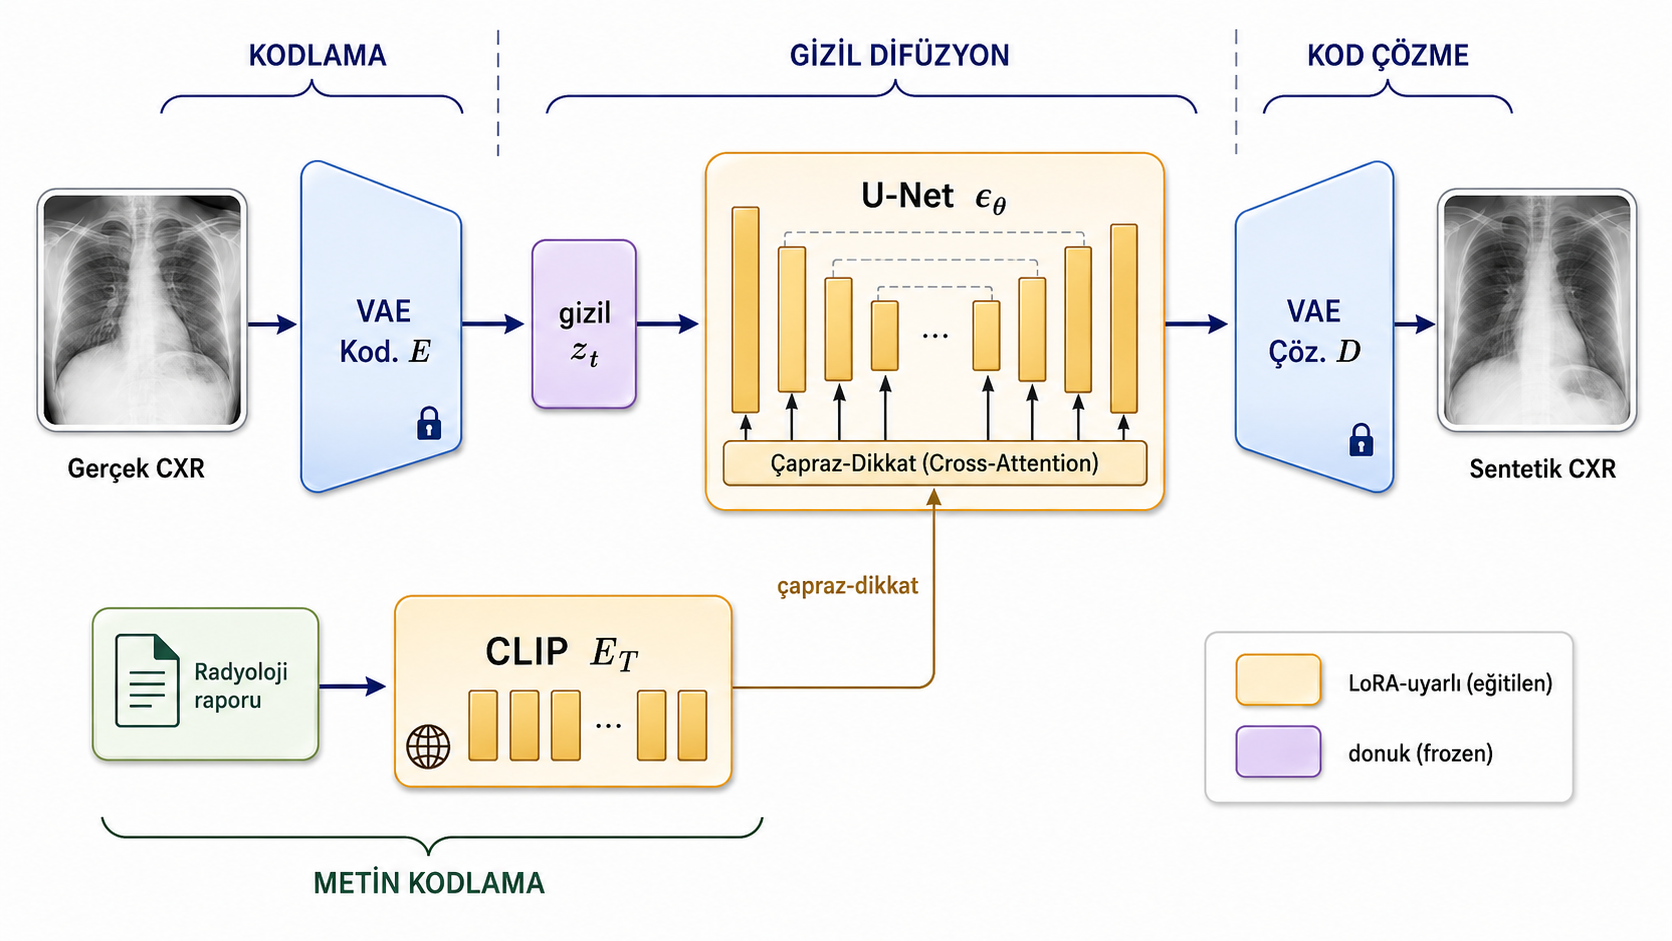
\includegraphics[width=\linewidth]{mimari.png}
\caption{Önerilen kaynak-verimli uyarlamanın mimari şeması. Radyoloji raporu
metni CLIP kodlayıcı ($E_T$) ile temsil edilip U-Net gürültü gidericisine
($\epsilon_\theta$) çapraz-dikkat yoluyla aktarılır ve üretimi koşullandırır.
Eğitimde gerçek CXR görüntüsü VAE kodlayıcı ($E$) ile gizil temsile ($z$)
dönüştürülürken, çıkarımda gizil temsil saf gürültüden başlatılır ve gerçek
görüntü kullanılmaz. Şekilde turuncu ile gösterilen ve U-Net ile $E_T$'nin
dikkat projeksiyon katmanlarına eklenen düşük-rank LoRA adapterleri eğitilir;
mor ile gösterilen VAE kodlayıcı/çözücü ($E$, $D$) ve taban ağırlıklar
dondurulur. Giderilen gizil temsil VAE çözücü ($D$) ile görüntü uzayına
çözülerek sentetik CXR elde edilir.}
\label{fig:arch}
\end{figure}

\begin{algorithm}[htbp]
\caption{LoRA ile kaynak-verimli CXR alan uyarlaması}
\label{alg:lora}
\begin{algorithmic}[1]
\Require Önceden eğitilmiş Stable Diffusion bileşenleri $(E,\epsilon_\theta,E_T,D)$;
CXR--metin çiftleri $\{(x_i,c_i)\}$; rank $r$; ölçek katsayısı $\alpha$;
öğrenme oranı $\eta$; eğitim adımı $S$
\State VAE bileşenlerini ve taban model ağırlıklarını dondur
\State U-Net ve metin kodlayıcının hedef dikkat katmanlarına LoRA matrisleri
$A$ ve $B$ ekle
\State $B$ matrislerini sıfırla başlat; eğitilebilir parametre kümesini
$\Theta \gets \{A,B\}$ olarak tanımla
\For{$s=1$ \textbf{to} $S$}
    \State Bir mini-grup $(x,c)$ örnekle
    \State $z_0 \gets E(x)$
    \State $t \sim \mathcal{U}\{1,\dots,T\}$ ve
    $\epsilon \sim \mathcal{N}(0,I)$ örnekle
    \State $z_t \gets \sqrt{\bar\alpha_t}z_0 +
    \sqrt{1-\bar\alpha_t}\epsilon$
    \State $\hat{\epsilon} \gets
    \epsilon_\theta\big(z_t,t,E_T(c)\big)$
    \State $\mathcal{L} \gets \|\epsilon-\hat{\epsilon}\|_2^2$
    \State $\Theta \gets \Theta - \eta \nabla_\Theta \mathcal{L}$
\EndFor
\State LoRA ağırlıklarını taban ağırlıklarla birleştir:
$W \leftarrow W_0 + \frac{\alpha}{r}BA$
\State \Return Alan-uyarlanmış model
\end{algorithmic}
\end{algorithm}

\subsection{İncelenen Ablasyon Varyantları}

Kaynak-kısıtlı eğitim rejiminde farklı tasarım tercihlerinin etkisini analiz
etmek amacıyla üç temel ablasyon varyantı incelenmiştir. Bu ablasyonlar,
LoRA tabanlı temel uyarlama yaklaşımının hangi koşullarda avantaj sağladığını
ve hangi durumlarda sınırlı kalabileceğini değerlendirmek için tasarlanmıştır.

\subsubsection{Üretim Çözünürlüğünün Artırılması}

İlk ablasyon, üretim çözünürlüğünün 256$\times$256'dan 512$\times$512'ye
çıkarılmasının etkisini incelemektedir. Daha yüksek çözünürlük, teorik olarak
daha ince anatomik ayrıntıların ve radyografik yapıların temsil edilmesine
olanak sağlayabilir. Bununla birlikte, çözünürlüğün artması difüzyon modelinin
öğrenmesi gereken dağılımı daha karmaşık hale getirmekte ve aynı eğitim adımı
sayısı altında yakınsamayı zorlaştırabilmektedir.

LoRA'nın bellek avantajı sayesinde 512$\times$512 çözünürlükte eğitim tek-GPU
kısıtı altında mümkün hale gelmiştir. Ancak bu ablasyonun amacı yalnızca daha
yüksek çözünürlüğün teknik olarak uygulanabilirliğini göstermek değil, sabit
eğitim bütçesi altında çözünürlük artışının üretim kalitesine gerçekten katkı
sağlayıp sağlamadığını değerlendirmektir.

\subsubsection{Rank-Kararlı LoRA Ölçeklemesi}

İkinci ablasyon, yüksek rank değerlerinde LoRA eğitiminin kararlılığını
artırmayı amaçlayan rank-kararlı LoRA ölçeklemesini incelemektedir~\cite{rslora}.
Standart LoRA'da güncelleme ölçeği $\alpha/r$ biçiminde tanımlanırken,
rsLoRA yaklaşımı bu ölçeklemeyi $\alpha/\sqrt{r}$ olarak yeniden düzenler.
Bu değişiklik, özellikle rank değeri arttığında gradyan büyüklüğünün aşırı
azalmasını önlemeyi ve daha kararlı bir eğitim süreci sağlamayı hedefler.

Bu çalışmada rsLoRA, daha yüksek rank değerinin üretim çeşitliliği ve alan-içi
sadakat üzerindeki etkisini incelemek amacıyla kullanılmıştır. Böylece yalnızca
daha fazla düşük-rank kapasite eklemenin kaynak-kısıtlı eğitim rejiminde kalite
artışı sağlayıp sağlamadığı değerlendirilebilmiştir.

\subsubsection{Patoloji-Ödül Tabanlı Ek Kayıp}

Üçüncü ablasyon, üretilen görüntülerin metin istemlerinde belirtilen patolojik
bulgularla daha uyumlu hale getirilmesini hedefleyen patoloji-ödül tabanlı ek
kayıp bileşenini incelemektedir. Bu amaçla, göğüs röntgenleri üzerinde
önceden eğitilmiş ve eğitim sırasında dondurulmuş bir sınıflandırıcı
$C$ kullanılmıştır~\cite{xrv}. Modelin tahmin ettiği temiz görüntü
$\hat{x}_0$, bu sınıflandırıcıya verilerek patoloji olasılıkları elde edilmiş
ve bu olasılıklar CheXpert etiketleriyle ikili çapraz entropi kaybı üzerinden
karşılaştırılmıştır.

Patoloji-ödül varyantında toplam kayıp fonksiyonu aşağıdaki şekilde
tanımlanmıştır:
\begin{equation}
\mathcal{L} =
\mathcal{L}_{\text{MSE}} +
\lambda \,
\text{BCE}\big(C(\hat{x}_0), y\big),
\label{eq:prg_loss}
\end{equation}
burada $\lambda$ patoloji-ödül bileşeninin ağırlığını, $y$ ise hedef patoloji
etiketlerini ifade etmektedir. Tahmin edilen temiz görüntü $\hat{x}_0$,
modelin gürültü tahmininden aşağıdaki şekilde yaklaşık olarak elde edilmiştir:
\begin{equation}
\hat{x}_0 =
D\left(
\frac{
z_t - \sqrt{1-\bar\alpha_t}\hat{\epsilon}
}{
\sqrt{\bar\alpha_t}
}
\right).
\label{eq:x0_prediction}
\end{equation}

Bu ablasyon, patolojiye duyarlı ek bir denetim sinyalinin üretim sürecine
katkı sağlayıp sağlamadığını değerlendirmek amacıyla tasarlanmıştır. Bununla
birlikte, bu tür ödül tabanlı sinyallerin difüzyonun temel gürültü giderme
hedefiyle etkileşimi dikkatli biçimde ele alınmalıdır. Özellikle yüksek gürültü
seviyelerinde $\hat{x}_0$ tahmininin kararsız olması, sınıflandırıcıdan gelen
gradyanın üretim sadakati üzerinde olumsuz etki oluşturmasına neden olabilir.
Bu nedenle patoloji-ödül bileşeni, çalışmanın ana yöntemi olarak değil,
kontrollü bir ablasyon varyantı olarak değerlendirilmiştir.

\subsection{Yöntemsel Karşılaştırmanın Kapsamı}

Bu çalışmadaki yöntemsel karşılaştırma, mutlak olarak en yüksek üretim kalitesini
elde etmekten ziyade, aynı kaynak kısıtları altında farklı uyarlama
stratejilerinin davranışını analiz etmeyi amaçlamaktadır. Bu nedenle tüm
modeller aynı veri alt kümesi, aynı eğitim adımı sayısı ve aynı değerlendirme
protokolü altında incelenmiştir. Böylece gözlenen farkların büyük ölçüde
uyarlama stratejisinden, eğitilebilir parametre sayısından ve kaynak kullanım
profilinden kaynaklanması hedeflenmiştir.

Tam ince ayar yaklaşımı yüksek uyarlama kapasitesi sunarken, bellek kullanımı
nedeniyle düşük etkin toplu boyutuyla sınırlı kalmaktadır. LoRA ise daha az
eğitilebilir parametreyle çalışmasına rağmen daha düşük bellek kullanımı ve daha
yüksek etkin toplu boyutu sağlayarak farklı bir optimizasyon rejimi
oluşturmaktadır. Bu karşılaştırma, kaynak-kısıtlı metin-koşullu tıbbi görüntü
üretiminde model kapasitesi, bellek verimliliği ve yakınsama arasındaki ilişkiyi
daha açık biçimde değerlendirmeyi mümkün kılmaktadır.


% ============================================================================
\section{Deneysel Kurulum}
\label{sec:setup}
% ============================================================================

Bu bölümde, çalışmada kullanılan veri kümesi, ön işleme adımları, eğitim
konfigürasyonları, donanım ortamı ve değerlendirme metrikleri açıklanmaktadır.
Tüm deneyler, tam ince ayar ve LoRA tabanlı parametre-verimli uyarlama
yaklaşımlarının tek-GPU kısıtı altında karşılaştırılmasına olanak sağlayacak
şekilde tasarlanmıştır. Bu nedenle modeller aynı veri alt kümesi, aynı eğitim
adımı sayısı ve aynı değerlendirme protokolü altında incelenmiştir.

\subsection{Veri Kümesi}

Deneylerde MIMIC-CXR v2.0.0 veri kümesi kullanılmıştır~\cite{mimic}. MIMIC-CXR,
göğüs röntgeni görüntüleri ile bu görüntülere ait serbest metin radyoloji
raporlarını içeren geniş ölçekli ve kimliksizleştirilmiş bir veri kümesidir.
Metin-koşullu görüntü üretimi için uygun yapısı nedeniyle, Stable Diffusion
modelinin göğüs röntgeni alanına uyarlanmasında tercih edilmiştir.

RoentGen çalışmasıyla tutarlı bir deneysel çerçeve oluşturmak amacıyla yalnızca
posterior--anterior (PA) projeksiyonlu göğüs röntgenleri kullanılmıştır. PA
projeksiyonunun seçilmesi, görüntüleme geometrisinden kaynaklanabilecek
varyasyonu azaltmak ve modelin daha homojen bir görüntü dağılımı üzerinde
eğitilmesini sağlamak amacı taşımaktadır. Lateral veya farklı projeksiyonlara
ait görüntüler bu çalışmanın kapsamı dışında bırakılmıştır.

Metin koşulu olarak radyoloji raporlarının \emph{impression} bölümü
kullanılmıştır. Bu bölüm, radyolojik bulguların özetlendiği ve klinik açıdan
en belirleyici ifadelerin yer aldığı kısım olduğundan, metin-koşullu üretim
için uygun bir denetim sinyali sağlamaktadır. Çok kısa veya modelin metin
kodlayıcısı tarafından işlenemeyecek kadar uzun raporlar veri kümesinden
çıkarılmıştır. Bu kapsamda, 7 karakterden kısa metinler ve CLIP
belirteçleyicisinin 77 belirteçlik giriş sınırını aşan örnekler elenmiştir.

Eğitim ve değerlendirme ayrımı hasta düzeyinde ayrışmayı koruyacak şekilde
oluşturulmuştur. Eğitim için \texttt{p10--p18} klasörlerindeki örnekler,
değerlendirme için ise \texttt{p19} klasöründeki örnekler kullanılmıştır.
Bu tercih, eğitim ve test aşamalarında aynı hastaya ait görüntülerin
karışmasını önlemeyi ve değerlendirme sonuçlarının daha güvenilir olmasını
amaçlamaktadır.

\subsection{Veri Ön İşleme}

Görüntüler eğitimden önce standart bir ön işleme hattından geçirilmiştir. İlk
olarak, her görüntü hedef çözünürlüğe uygun olacak şekilde kısa kenar üzerinden
yeniden ölçeklenmiştir. Ardından, görüntülerin kare formata getirilmesi için
merkezi kırpma uygulanmıştır. Bu işlem, modelin giriş boyutuyla uyumlu
sabit boyutlu görüntüler elde edilmesini sağlamaktadır.

Kırpma ve yeniden boyutlandırma işlemlerinin ardından görüntü piksel değerleri
$[-1,1]$ aralığına normalleştirilmiştir. Bu normalizasyon, Stable Diffusion
modelinin VAE kodlayıcısı tarafından beklenen giriş aralığıyla uyumludur.
Eğitim sırasında görüntüler VAE kodlayıcı aracılığıyla gizil uzaya
aktarılmış ve difüzyon süreci bu gizil temsil üzerinde yürütülmüştür.

Metin verileri CLIP belirteçleyicisi kullanılarak işlenmiştir. Her metin istemi,
CLIP metin kodlayıcısının giriş yapısına uygun olacak şekilde en fazla 77
belirtece dönüştürülmüştür. Daha kısa metinler sabit uzunluğu sağlamak amacıyla
doldurulmuş, sınırı aşan metinler ise veri kümesinden çıkarılmıştır. Böylece
hem görüntü hem de metin verileri Stable Diffusion mimarisiyle uyumlu hale
getirilmiştir.

\subsection{Eğitim Konfigürasyonları}

Tüm modeller, adil bir karşılaştırma sağlamak amacıyla aynı genel eğitim
bütçesi altında eğitilmiştir. Deneylerde Stable Diffusion v1.4 taban model
olarak kullanılmıştır. Tam ince ayar yaklaşımında VAE bileşeni dondurulmuş,
U-Net ve CLIP metin kodlayıcısı birlikte eğitilmiştir. LoRA tabanlı
yaklaşımlarda ise taban model ağırlıkları dondurulmuş ve yalnızca hedef dikkat
projeksiyon katmanlarına eklenen düşük-rank adapter parametreleri
güncellenmiştir.

Eğitim sürecinde AdamW optimizasyon yöntemi kullanılmış ve gradyan normu
1,0 değeriyle sınırlandırılmıştır. Tam ince ayar için öğrenme oranı
$5\times10^{-5}$, LoRA tabanlı deneyler için ise $1\times10^{-4}$ olarak
belirlenmiştir. Tüm modeller 5000 eğitim adımı boyunca eğitilmiş ve aynı
5000 PA örnekten oluşan veri alt kümesi kullanılmıştır. Eğitim sürecinde
bfloat16 otomatik karma hassasiyet kullanılmış, ana ağırlıklar ise fp32 olarak
korunmuştur.

Temel deneylerde görüntü çözünürlüğü 256$\times$256 olarak belirlenmiştir.
Çözünürlük ablasyonu kapsamında LoRA modeli ayrıca 512$\times$512 çözünürlükte
eğitilmiştir. Standart LoRA deneyinde rank değeri $r=8$ ve ölçek katsayısı
$\alpha=8$ olarak kullanılmıştır. rsLoRA ablasyonunda ise rank değeri $r=16$
olarak belirlenmiştir. LoRA adapterleri U-Net ve CLIP metin kodlayıcısındaki
\texttt{to\_q}, \texttt{to\_k}, \texttt{to\_v} ve \texttt{to\_out}
projeksiyonlarına uygulanmıştır.

\begin{table}[htbp]
\centering
\caption{Eğitim ve uyarlama hiperparametreleri.}
\label{tab:hp}
\small
\begin{tabular}{@{}ll@{}}
\toprule
\textbf{Bileşen} & \textbf{Değer} \\
\midrule
Taban model & Stable Diffusion v1.4 \\
Veri kümesi & MIMIC-CXR v2.0.0, PA projeksiyonları \\
Metin koşulu & Raporların \emph{impression} bölümü \\
Eğitim örnekleri & 5000 PA örnek \\
Eğitim adımı & 5000 \\
Optimizasyon & AdamW, gradyan kırpma 1,0 \\
Öğrenme oranı & $5\times10^{-5}$ (tam ince ayar), $1\times10^{-4}$ (LoRA) \\
Hassasiyet & bfloat16 autocast, fp32 master ağırlık \\
Temel çözünürlük & 256$\times$256 \\
Çözünürlük ablasyonu & 512$\times$512 \\
LoRA rank / $\alpha$ & 8 / 8 \\
rsLoRA rank & 16 \\
LoRA hedef katmanları & \texttt{to\_q}, \texttt{to\_k}, \texttt{to\_v}, \texttt{to\_out} \\
Çıkarım ayarı & DDIM, 20 adım, CFG 4,0 \\
Donanım & Tek GPU, 24 GB VRAM \\
\bottomrule
\end{tabular}
\end{table}

\subsection{Karşılaştırılan Modeller}

Deneysel değerlendirme kapsamında beş farklı model konfigürasyonu
karşılaştırılmıştır. İlk model, tam ince ayar yaklaşımını temsil eden baseline
modeldir. Bu modelde U-Net ve CLIP metin kodlayıcısı birlikte eğitilmiş, VAE
dondurulmuştur. İkinci model, 256$\times$256 çözünürlükte eğitilen standart
LoRA konfigürasyonudur. Bu model, çalışmanın temel parametre-verimli uyarlama
yaklaşımını oluşturmaktadır.

Üçüncü model, LoRA tabanlı patoloji-ödül varyantıdır. Bu modelde standart MSE
gürültü tahmin kaybına ek olarak, dondurulmuş bir göğüs röntgeni
sınıflandırıcısından elde edilen patoloji uyum kaybı eklenmiştir. Dördüncü
model, LoRA'nın 512$\times$512 çözünürlükte eğitilen versiyonudur. Beşinci
model ise 512$\times$512 çözünürlükte, rank-kararlı ölçekleme kullanan
rsLoRA varyantıdır.

\begin{table}[htbp]
\centering
\caption{Deneylerde karşılaştırılan model konfigürasyonları.}
\label{tab:models}
\small
\begin{tabular}{@{}l l c >{\raggedright\arraybackslash}p{0.34\textwidth}@{}}
\toprule
\textbf{Model} & \textbf{Uyarlama yöntemi} & \textbf{Çözünürlük} & \textbf{Açıklama} \\
\midrule
Baseline & Tam ince ayar & 256$\times$256 &
U-Net ve CLIP metin kodlayıcı birlikte eğitilir \\

LoRA & Parametre-verimli uyarlama & 256$\times$256 &
U-Net ve CLIP dikkat katmanlarına LoRA uygulanır \\

PRG & LoRA + patoloji-ödül & 256$\times$256 &
MSE kaybına ek patoloji uyum kaybı eklenir \\

LoRA-512 & Parametre-verimli uyarlama & 512$\times$512 &
Yüksek çözünürlükte LoRA eğitimi \\

rsLoRA-512 & Rank-kararlı LoRA & 512$\times$512 &
$r=16$ ve $\alpha/\sqrt{r}$ ölçeklemesi kullanılır \\
\bottomrule
\end{tabular}
\end{table}

\subsection{Çıkarım Protokolü}

Eğitim tamamlandıktan sonra tüm modeller aynı çıkarım protokolüyle
değerlendirilmiştir. Böylece üretim kalitesindeki farkların çıkarım
ayarlarından değil, eğitim ve uyarlama stratejisinden kaynaklanması
hedeflenmiştir. Görüntü üretimi için DDIM çizelgeleyici kullanılmış, gürültü
giderme adım sayısı 20 olarak belirlenmiştir. Sınıflandırıcısız rehberlik
ölçeği (classifier-free guidance, CFG) 4,0 olarak ayarlanmıştır.

Test aşamasında, değerlendirme kümesinden seçilen radyolojik metin istemleri
modele verilmiş ve her istem için sentetik göğüs röntgeni görüntüleri
üretilmiştir. 256 çözünürlükte eğitilen modeller 256$\times$256, 512
çözünürlükte eğitilen modeller ise 512$\times$512 çözünürlükte görüntü
üretmiştir. Bu tercih, her modelin kendi eğitim çözünürlüğünde
değerlendirilmesini sağlamaktadır.

\subsection{Değerlendirme Metrikleri}

Üretilen görüntülerin kalitesi, dağılım uyumu, alan-içi sadakat, çeşitlilik ve
metin--görüntü hizalaması açısından değerlendirilmiştir. Bu amaçla dört temel
metrik kullanılmıştır: FID, FID$_{\text{XRV}}$, MS-SSIM ve CLIP-sim. Tüm
metrikler 200 test örneği üzerinde hesaplanmıştır.

\textbf{FID.} Fréchet Inception Distance (FID), gerçek ve üretilen görüntülerin
InceptionV3 öznitelik uzayındaki dağılımları arasındaki mesafeyi ölçmektedir
\cite{fid}. Daha düşük FID değeri, üretilen görüntü dağılımının gerçek görüntü
dağılımına daha yakın olduğunu gösterir. Bu çalışmada FID hesaplamasında
yeniden boyutlandırma ve ön işleme farklılıklarından kaynaklanabilecek
sapmaları azaltmak amacıyla clean-fid yaklaşımı kullanılmıştır~\cite{cleanfid}.

\textbf{FID$_{\text{XRV}}$.} Genel amaçlı FID metriği ImageNet üzerinde
eğitilmiş InceptionV3 özniteliklerine dayandığından, göğüs röntgenleri gibi
tıbbi görüntüler için sınırlı temsil gücüne sahip olabilir. Bu nedenle,
alan-içi sadakati değerlendirmek için göğüs röntgenleri üzerinde önceden
eğitilmiş DenseNet-121 tabanlı TorchXRayVision modeli kullanılarak
FID$_{\text{XRV}}$ hesaplanmıştır~\cite{xrv}. Daha düşük FID$_{\text{XRV}}$
değeri, üretilen görüntülerin göğüs röntgeni alanındaki gerçek görüntü
dağılımına daha yakın olduğunu göstermektedir.

\textbf{MS-SSIM.} Üretim çeşitliliğini değerlendirmek amacıyla çok-ölçekli
yapısal benzerlik indeksi (MS-SSIM) kullanılmıştır. Aynı veya benzer istemler
için üretilen görüntüler arasındaki yapısal benzerliğin düşük olması, modelin
daha çeşitli örnekler üretebildiğine işaret eder. Bu nedenle MS-SSIM metriğinde
daha düşük değerler daha yüksek çeşitlilik olarak yorumlanmıştır.

\textbf{CLIP-sim.} Metin--görüntü hizalamasını değerlendirmek için CLIP tabanlı
kosinüs benzerliği kullanılmıştır. Bu metrik, üretilen görüntü ile ilgili metin
istemi arasındaki semantik uyumu ölçmeyi amaçlar. Daha yüksek CLIP-sim değeri,
metin koşulunun üretim sürecine daha iyi yansıtıldığını göstermektedir. Ancak
CLIP'in doğal görüntü--metin çiftleri üzerinde eğitilmiş olması nedeniyle,
bu metrik tıbbi alanda tamamlayıcı bir gösterge olarak değerlendirilmiştir.

\subsection{Deneysel Tasarımın Kapsamı ve Sınırlılıkları}

Bu deneysel kurulum, tam ince ayar ve parametre-verimli uyarlama stratejilerinin
tek-GPU kısıtı altında göreli davranışlarını karşılaştırmayı amaçlamaktadır.
Dolayısıyla çalışmanın temel hedefi, en yüksek mutlak üretim kalitesine ulaşmak
değil, aynı veri ve eğitim bütçesi altında farklı uyarlama stratejilerinin
kalite--verimlilik dengesini analiz etmektir.

Bu kapsamda kullanılan eğitim alt kümesi, eğitim adımı sayısı ve test örneği
sayısı bilinçli olarak sabit tutulmuştur. Bu tercih, modeller arası adil bir
karşılaştırma yapılmasını sağlasa da, sonuçların daha büyük veri kümeleri,
daha uzun eğitim süreleri veya farklı donanım konfigürasyonları altında
değişebileceği göz önünde bulundurulmalıdır. Bu nedenle elde edilen bulgular,
çalışmada tanımlanan kaynak-kısıtlı deneysel koşullar bağlamında
yorumlanmalıdır.


% ============================================================================
\section{Bulgular}
\label{sec:results}
% ============================================================================

Bu bölümde, tam ince ayar ve LoRA tabanlı parametre-verimli uyarlama
yaklaşımlarının tek-GPU kısıtı altındaki deneysel sonuçları sunulmaktadır.
Sonuçlar iki ana açıdan değerlendirilmiştir: kaynak kullanımı ve üretim
kalitesi. Kaynak kullanımı kapsamında eğitilebilir parametre sayısı, tepe GPU
bellek tüketimi ve eğitim süresi karşılaştırılmıştır. Üretim kalitesi ise genel
FID, alan-içi FID$_{\text{XRV}}$, MS-SSIM ve CLIP-sim metrikleri üzerinden
incelenmiştir. Tüm sonuçlar, çalışmada tanımlanan sabit veri alt kümesi, eğitim
adımı ve değerlendirme protokolü altında yorumlanmalıdır.

\subsection{Kaynak Kullanımı ve Eğitim Verimliliği}

Tablo~\ref{tab:eff}, karşılaştırılan modellerin kaynak kullanımı ve eğitim
verimliliği sonuçlarını göstermektedir. Tam ince ayar yaklaşımı, U-Net ve CLIP
metin kodlayıcısının birlikte eğitilmesi nedeniyle 982,6 milyon eğitilebilir
parametre içermektedir. Bu değer, model parametrelerinin yaklaşık \%92,2'sinin
eğitim sırasında güncellendiğini göstermektedir. Buna karşılık standart LoRA
konfigürasyonu yalnızca 2,18 milyon eğitilebilir parametre kullanmaktadır. Bu,
toplam model parametrelerinin yaklaşık \%0,20'sine karşılık gelmektedir.

\begin{table}[htbp]
\centering
\caption{Sabit eğitim bütçesi altında kaynak kullanımı ve eğitim verimliliği.}
\label{tab:eff}
\small
\begin{tabular}{@{}lccccc@{}}
\toprule
\textbf{Model} & \textbf{Çöz.} & \textbf{Etkin batch} & \textbf{Eğit.\ par.} &
\textbf{Tepe VRAM} & \textbf{Süre} \\
\midrule
Baseline (tam ince ayar) & 256 & 2  & 982,6M\ (\%92,2) & 20,1\,GB & 336,8\,dk \\
\textbf{LoRA} (r=8)      & 256 & 32 & 2,18M\ (\%0,20)  & \textbf{3,0\,GB} & \textbf{118,8\,dk} \\
PRG (LoRA r=8 + ödül)    & 256 & 32 & 2,18M\ (\%0,20)  & 10,3\,GB & 144,7\,dk \\
LoRA (r=8)               & 512 & 32 & 2,18M\ (\%0,20)  & 4,0\,GB  & 372,7\,dk \\
LoRA + rsLoRA (r=16)     & 512 & 32 & 4,37M\ (\%0,41)  & 4,0\,GB  & 435,3\,dk \\
\bottomrule
\end{tabular}
\end{table}

Bellek kullanımı açısından LoRA tabanlı yaklaşım, tam ince ayara kıyasla belirgin
bir avantaj sağlamıştır. Tam ince ayar 256$\times$256 çözünürlükte 20,1 GB tepe
GPU belleği kullanırken, standart LoRA modeli aynı çözünürlükte 3,0 GB tepe
bellek ile eğitilebilmiştir. Bu sonuç, LoRA'nın optimizer durumunu yalnızca
düşük-rank adapter parametreleri için tutmasının bellek maliyetini önemli ölçüde
azalttığını göstermektedir. Bellek kullanımındaki bu azalma, aynı donanım
üzerinde daha yüksek etkin toplu boyutuyla eğitim yapılmasına da olanak
sağlamıştır. Tam ince ayar yaklaşımı etkin batch değeri 2 ile sınırlı kalırken,
LoRA tabanlı deneylerde etkin batch değeri 32 olarak kullanılmıştır.

Eğitim süresi bakımından da standart LoRA konfigürasyonu daha verimli bir
profil sergilemiştir. Tam ince ayar 336,8 dakikada tamamlanırken, LoRA modeli
118,8 dakikada eğitilmiştir. Bu sonuç, LoRA'nın yalnızca bellek tüketimini değil,
aynı zamanda eğitim süresini de azalttığını göstermektedir. Bununla birlikte,
çözünürlüğün 512$\times$512'ye çıkarılması eğitim süresini belirgin biçimde
artırmıştır. LoRA-512 modeli 372,7 dakikada, rsLoRA-512 modeli ise 435,3
dakikada eğitilmiştir. Bu durum, daha yüksek çözünürlüğün bellek açısından
mümkün hale gelmesine rağmen, hesaplama süresi bakımından ek maliyet oluşturduğunu
göstermektedir.

Patoloji-ödül tabanlı PRG varyantı, standart LoRA ile aynı sayıda eğitilebilir
parametreye sahip olmasına rağmen daha yüksek bellek kullanımı ve daha uzun
eğitim süresi gerektirmiştir. Bu artış, dondurulmuş göğüs röntgeni
sınıflandırıcısının ek ileri geçişleri ve patoloji-ödül kaybının hesaplanmasıyla
ilişkilidir. Dolayısıyla PRG varyantı, parametre sayısı bakımından LoRA ile aynı
olsa da, pratik eğitim maliyeti açısından daha ağır bir konfigürasyon
oluşturmuştur.

Genel olarak kaynak kullanımı sonuçları, LoRA tabanlı uyarlamanın tek-GPU
kısıtı altında tam ince ayara kıyasla daha elverişli bir eğitim profili sunduğunu
göstermektedir. Bu avantaj yalnızca daha az eğitilebilir parametreyle sınırlı
değildir; aynı zamanda daha düşük optimizer belleği, daha yüksek etkin toplu
boyutu ve daha kısa eğitim süresiyle de ilişkilidir.

\subsection{Nicel Üretim Kalitesi}

Tablo~\ref{tab:quality}, karşılaştırılan modellerin üretim kalitesi sonuçlarını
göstermektedir. Değerlendirme, 200 test örneği üzerinde FID,
FID$_{\text{XRV}}$, MS-SSIM ve CLIP-sim metrikleriyle gerçekleştirilmiştir.
Bu metrikler birlikte ele alındığında, standart LoRA konfigürasyonunun
kaynak-kısıtlı deneysel koşullarda en dengeli performansı sunduğu görülmektedir.

\begin{table}[htbp]
\centering
\caption{Üretim kalitesi karşılaştırması.}
\label{tab:quality}
\small
\begin{tabular}{@{}lcccc@{}}
\toprule
\textbf{Model} & \textbf{FID}~$\downarrow$ & \textbf{FID$_{\text{XRV}}$}~$\downarrow$
& \textbf{MS-SSIM}~$\downarrow$ & \textbf{CLIP-sim}~$\uparrow$ \\
\midrule
Baseline (tam ince ayar, 256) & 122,67 & 6,74  & 0,222 & 0,231 \\
\textbf{LoRA (r=8, 256)}      & \textbf{91,42} & \textbf{4,09} & 0,325 & 0,239 \\
PRG (LoRA + ödül, 256)        & 128,90 & 10,69 & 0,446 & 0,238 \\
LoRA (r=8, 512)               & 93,92  & 7,17  & 0,313 & \textbf{0,240} \\
LoRA + rsLoRA (r=16, 512)     & 124,19 & 9,26  & \textbf{0,177} & 0,234 \\
\bottomrule
\end{tabular}
\end{table}

Genel FID metriğinde en düşük değer standart LoRA modeli tarafından elde
edilmiştir. LoRA modeli 91,42 FID değeriyle tam ince ayar baseline'ından
daha iyi bir dağılım uyumu göstermiştir. Tam ince ayarın FID değeri 122,67
olarak ölçülmüştür. Bu sonuç, incelenen tek-GPU ve sabit eğitim bütçesi
koşullarında tam ince ayarın yüksek parametre kapasitesini etkili biçimde
kullanmakta zorlanmış olabileceğini düşündürmektedir.

Alan-içi FID$_{\text{XRV}}$ metriğinde de benzer bir eğilim gözlemlenmiştir.
Standart LoRA modeli 4,09 değeriyle en düşük FID$_{\text{XRV}}$ sonucunu
elde etmiştir. Tam ince ayar modeli ise 6,74 değerinde kalmıştır. Bu bulgu,
LoRA tabanlı uyarlamanın yalnızca genel görüntü öznitelikleri açısından değil,
göğüs röntgeni alanına özgü öznitelik dağılımı açısından da daha uygun sonuçlar
ürettiğini göstermektedir. Bununla birlikte, bu sonuç çalışmada kullanılan
veri alt kümesi, eğitim adımı ve tek-GPU kısıtı bağlamında yorumlanmalıdır.

Çözünürlüğün 512$\times$512'ye çıkarılması, standart LoRA modeline kıyasla
alan-içi FID değerinde iyileşme sağlamamıştır. LoRA-512 modeli 7,17
FID$_{\text{XRV}}$ değeriyle 256 çözünürlükteki LoRA modelinin gerisinde
kalmıştır. Bu sonuç, daha yüksek çözünürlüğün tek başına üretim kalitesini
artırmadığını; aynı zamanda yeterli eğitim süresi, veri miktarı ve yakınsama
koşulları gerektirdiğini göstermektedir. Benzer şekilde rsLoRA-512 modeli de
9,26 FID$_{\text{XRV}}$ değeriyle standart LoRA konfigürasyonunun gerisinde
kalmıştır.

PRG varyantı, patoloji-ödül bileşeninin eklenmesine rağmen üretim kalitesini
iyileştirmemiştir. Aksine, PRG modeli hem genel FID hem de FID$_{\text{XRV}}$
açısından en zayıf sonuçlardan birini vermiştir. PRG'nin FID$_{\text{XRV}}$
değeri 10,69 olarak ölçülmüştür. Bu durum, sınıflandırıcı tabanlı ek ödül
sinyalinin difüzyon modelinin temel gürültü giderme hedefiyle uyumlu
çalışmadığını ve kaynak-kısıtlı eğitim rejiminde üretim sadakatini olumsuz
etkileyebileceğini göstermektedir.

MS-SSIM sonuçları, modellerin üretim çeşitliliği açısından farklı davranışlar
sergilediğini göstermektedir. En düşük MS-SSIM değeri rsLoRA-512 modelinde
0,177 olarak ölçülmüştür. Bu değer, rsLoRA-512 modelinin daha çeşitli örnekler
üretebildiğine işaret etmektedir. Ancak aynı modelin FID ve
FID$_{\text{XRV}}$ değerlerinin yüksek olması, çeşitlilik artışının dağılım
sadakatiyle birlikte gerçekleşmediğini göstermektedir. Buna karşılık standart
LoRA modeli daha yüksek MS-SSIM değerine sahip olsa da, FID ve
FID$_{\text{XRV}}$ açısından daha güçlü sonuçlar vermiştir. Bu bulgu,
kaynak-kısıtlı koşullarda çeşitlilik ve sadakat arasında bir denge kurulması
gerektiğini göstermektedir.

CLIP-sim metriğinde modeller arasında büyük farklar gözlemlenmemiştir.
En yüksek CLIP-sim değeri 0,240 ile LoRA-512 modelinde elde edilmiştir.
Standart LoRA modeli ise 0,239 değeriyle oldukça yakın bir sonuç vermiştir.
Tam ince ayar modelinin CLIP-sim değeri 0,231 olarak ölçülmüştür. Bu sonuçlar,
LoRA tabanlı yaklaşımların metin--görüntü hizalaması açısından tam ince ayara
kıyasla daha iyi veya benzer düzeyde performans gösterebildiğini düşündürse de,
CLIP'in doğal görüntü--metin çiftleri üzerinde eğitilmiş olması nedeniyle bu
metrik tıbbi bağlamda tamamlayıcı bir gösterge olarak değerlendirilmelidir.

\subsection{Ablasyon Bulguları}

Ablasyon deneyleri, kaynak-kısıtlı eğitim rejiminde model kapasitesi, çözünürlük
ve ek denetim sinyallerinin etkisini daha ayrıntılı biçimde değerlendirmeyi
amaçlamaktadır. Sonuçlar, bu tür tasarım değişikliklerinin her zaman üretim
kalitesine olumlu katkı sağlamadığını göstermektedir.

İlk olarak, çözünürlüğün 256$\times$256'dan 512$\times$512'ye çıkarılması,
nitel olarak daha ince ayrıntıların ortaya çıkmasına katkıda bulunabilse de,
nicel metriklerde tutarlı bir iyileşme sağlamamıştır. LoRA-512 modeli genel
FID açısından standart LoRA'ya yakın bir değer üretmiş olsa da,
FID$_{\text{XRV}}$ bakımından geride kalmıştır. Bu durum, yüksek çözünürlükte
öğrenilmesi gereken dağılımın daha karmaşık hale geldiğini ve sabit eğitim
adımı altında yeterli yakınsamanın sağlanamamış olabileceğini göstermektedir.

İkinci olarak, rsLoRA varyantı üretim çeşitliliği açısından en iyi MS-SSIM
sonucunu elde etmiştir. Ancak bu çeşitlilik artışı, alan-içi sadakat
metriklerine olumlu yansımamıştır. Bu bulgu, daha yüksek rank değerinin ve
rank-kararlı ölçeklemenin sabit eğitim bütçesi altında doğrudan kalite artışı
sağlamadığını göstermektedir. rsLoRA'nın potansiyel avantajlarının ortaya
çıkabilmesi için daha uzun eğitim süresi veya farklı hiperparametre ayarları
gerekebilir.

Üçüncü olarak, PRG varyantı patoloji uyumunu artırmak amacıyla tasarlanmış
olmasına rağmen genel üretim sadakatini düşürmüştür. Bu sonuç, sınıflandırıcı
tabanlı ek kayıpların difüzyon eğitimiyle bütünleştirilmesinin dikkatli biçimde
tasarlanması gerektiğini göstermektedir. Özellikle rastgele zaman adımlarında
tahmin edilen temiz görüntü üzerinden hesaplanan patoloji kaybı, yüksek gürültü
seviyelerinde kararsız gradyanlara neden olmuş olabilir. Bu nedenle PRG
yaklaşımı, mevcut haliyle standart LoRA'ya kıyasla avantaj sağlamamıştır.

Genel olarak ablasyon sonuçları, kaynak-kısıtlı metin-koşullu CXR üretiminde
model kapasitesini veya denetim sinyalini artırmanın tek başına yeterli
olmadığını göstermektedir. Üretim kalitesi, kapasitenin nasıl tahsis edildiği,
modelin ne ölçüde yakınsadığı ve eğitim sinyallerinin temel denoising hedefiyle
ne kadar uyumlu olduğu tarafından belirlenmektedir.

\subsection{Nitel Sonuçlar}

Şekil~\ref{fig:qual}, aynı radyolojik istem için farklı modeller tarafından
üretilen örnek görüntüleri göstermektedir. Nitel karşılaştırma, nicel metriklerde
gözlemlenen eğilimlerle genel olarak uyumludur. Tam ince ayar baseline modeli,
sınırlı eğitim bütçesi altında anatomik olarak daha bozulmuş ve yapısal açıdan
daha az tutarlı çıktılar üretmiştir. Bu durum, düşük etkin toplu boyutu ve
yüksek eğitilebilir parametre sayısının tek-GPU koşullarında optimizasyonu
zorlaştırmasıyla ilişkili olabilir.

Standart LoRA modeli, daha dengeli ve anatomik olarak daha tutarlı göğüs
röntgeni örnekleri üretmiştir. Görüntülerde genel toraks yapısı, akciğer
alanlarının simetrisi ve radyografik görünüm baseline'a kıyasla daha kararlı
görünmektedir. Bu nitel gözlem, LoRA modelinin FID ve FID$_{\text{XRV}}$
metriklerinde elde ettiği daha düşük değerlerle uyumludur.

512 çözünürlükte eğitilen LoRA modeli, bazı örneklerde daha ince görsel
ayrıntılar üretebilmiştir. Bununla birlikte, bu ayrıntı artışı nicel alan-içi
sadakat metriğine tutarlı biçimde yansımamıştır. PRG ve rsLoRA varyantlarında
ise bazı görüntülerde bulanıklık, düşük kontrast veya dağılım uyumunu
zayıflatabilecek görsel bozulmalar gözlemlenmiştir. Bu durum, söz konusu
varyantların standart LoRA'ya göre daha yüksek FID$_{\text{XRV}}$ değerleriyle
uyumludur.

\begin{figure}[htbp]
\centering
\begin{subfigure}{0.19\textwidth}
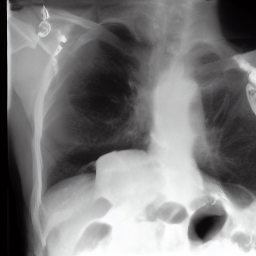
\includegraphics[width=\linewidth]{baseline.png}
\caption{Baseline}
\end{subfigure}\hfill
\begin{subfigure}{0.19\textwidth}
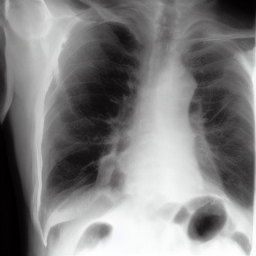
\includegraphics[width=\linewidth]{lora256.png}
\caption{LoRA 256}
\end{subfigure}\hfill
\begin{subfigure}{0.19\textwidth}
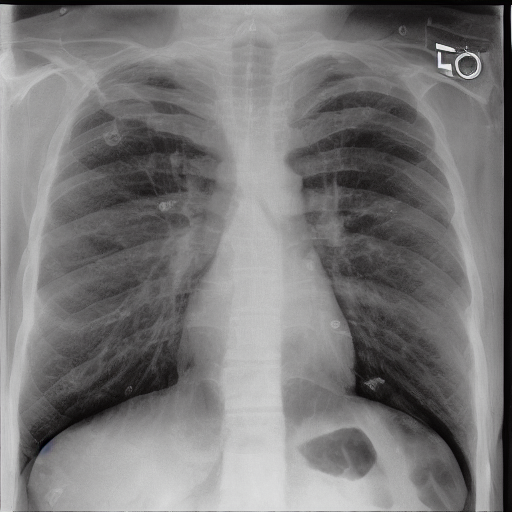
\includegraphics[width=\linewidth]{lora512.png}
\caption{LoRA 512}
\end{subfigure}\hfill
\begin{subfigure}{0.19\textwidth}
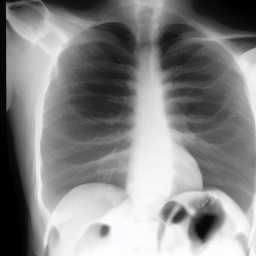
\includegraphics[width=\linewidth]{prg.png}
\caption{PRG}
\end{subfigure}\hfill
\begin{subfigure}{0.19\textwidth}
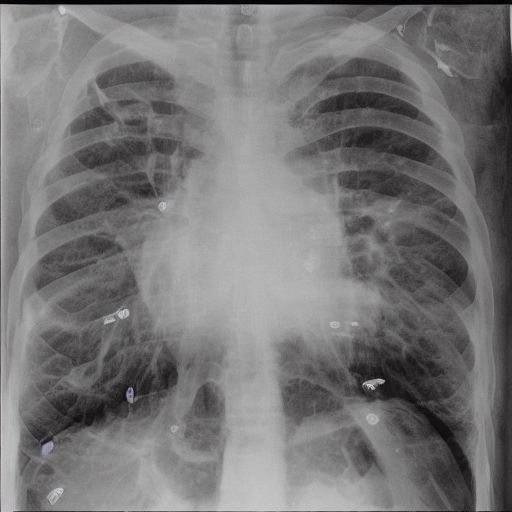
\includegraphics[width=\linewidth]{rslora512.png}
\caption{rsLoRA 512}
\end{subfigure}
\caption{Aynı radyolojik istem için farklı modeller tarafından üretilen örnek
görüntüler. Nitel sonuçlar, standart LoRA konfigürasyonunun kaynak-kısıtlı
eğitim koşullarında daha dengeli ve anatomik olarak daha tutarlı çıktılar
ürettiğini göstermektedir.}
\label{fig:qual}
\end{figure}

\subsection{Genel Değerlendirme}

Bulgular genel olarak değerlendirildiğinde, standart LoRA konfigürasyonu
tek-GPU ve sabit eğitim bütçesi altında en dengeli kalite--verimlilik profilini
sunmuştur. Tam ince ayar daha yüksek temsil kapasitesine sahip olmasına rağmen,
yüksek bellek kullanımı nedeniyle düşük etkin toplu boyutuyla sınırlı kalmış ve
bu deneysel koşullarda LoRA'nın gerisinde sonuçlar üretmiştir. LoRA ise çok daha
az eğitilebilir parametreyle çalışmasına rağmen daha düşük bellek kullanımı,
daha yüksek etkin toplu boyutu ve daha iyi alan-içi FID değeri sağlamıştır.

Ablasyon sonuçları, daha yüksek çözünürlük, daha yüksek rank veya ek patoloji
ödül sinyali gibi tasarım seçeneklerinin sabit eğitim bütçesi altında otomatik
olarak kalite artışı sağlamadığını göstermektedir. Bu bulgu, kaynak-kısıtlı
tıbbi difüzyon modeli uyarlamasında temel meselenin yalnızca model kapasitesini
artırmak değil, mevcut kapasitenin uygun biçimde tahsis edilmesi ve modelin
yeterli yakınsama koşullarında eğitilmesi olduğunu göstermektedir.


% ============================================================================
\section{Tartışma}
\label{sec:discussion}
% ============================================================================

Bu çalışma, metin-koşullu latent difüzyon modellerinin göğüs röntgeni alanına
uyarlanmasında tam ince ayar ve LoRA tabanlı parametre-verimli uyarlama
yaklaşımlarını tek-GPU kısıtı altında karşılaştırmıştır. Bulgular, incelenen
sabit veri, eğitim adımı ve donanım koşullarında LoRA tabanlı uyarlamanın tam
ince ayara kıyasla daha elverişli bir kalite--verimlilik dengesi sunduğunu
göstermektedir. Bu sonuç, parametre-verimli ince ayarın yalnızca daha düşük
maliyetli bir alternatif olmadığını; aynı zamanda kaynak-kısıtlı eğitim
rejiminde optimizasyon dinamiklerini değiştiren önemli bir strateji
olabileceğini göstermektedir.

\subsection{LoRA'nın Kaynak-Kısıtlı Rejimdeki Avantajı}

Tam ince ayar yaklaşımı, teorik olarak yüksek uyarlama kapasitesi sunmasına
rağmen, tek-GPU koşullarında önemli bellek kısıtlarıyla karşılaşmıştır. U-Net ve
CLIP metin kodlayıcısının birlikte eğitilmesi, çok sayıda eğitilebilir parametre
ve buna bağlı optimizer durumu gerektirdiğinden, tam ince ayar düşük etkin toplu
boyutuyla sınırlı kalmıştır. Bu durum, yalnızca donanım maliyetini artırmakla
kalmamakta, aynı zamanda gradyan tahmininin daha gürültülü hale gelmesine ve
optimizasyon sürecinin daha kırılgan olmasına neden olabilmektedir.

LoRA ise önceden eğitilmiş ağırlıkları dondurarak yalnızca düşük-rank adapter
parametrelerini eğitmektedir. Bu yapı, eğitilebilir parametre sayısını büyük
ölçüde azaltmakta ve optimizer belleğini sınırlamaktadır. Bulgularda görüldüğü
üzere, LoRA'nın bellek avantajı aynı donanım üzerinde daha yüksek etkin toplu
boyutuyla eğitim yapılmasını mümkün kılmıştır. Bu nedenle LoRA'nın avantajı
yalnızca parametre sayısının azalmasıyla açıklanmamalıdır. Daha düşük bellek
kullanımı, daha yüksek etkin batch değeri ve daha kararlı gradyan tahmini
birlikte değerlendirildiğinde, LoRA kaynak-kısıtlı senaryoda daha uygun bir
optimizasyon rejimi sağlamış olabilir.

Bu bulgu, tıbbi görüntü üretimi açısından önemlidir. Çünkü birçok araştırma
grubu veya klinik kurum, RoentGen gibi yüksek kaynaklı çalışmaların kullandığı
ölçekte GPU altyapısına sahip değildir. Dolayısıyla metin-koşullu tıbbi
difüzyon modellerinin pratikte yaygınlaşabilmesi için yalnızca yüksek üretim
kalitesine değil, aynı zamanda erişilebilir donanımlarda eğitilebilirliğe de
ihtiyaç vardır. Bu çalışmadaki sonuçlar, LoRA tabanlı uyarlamanın bu açıdan
uygulanabilir bir ara çözüm sunduğunu göstermektedir.

\subsection{Model Kapasitesi ve Yakınsama Arasındaki Denge}

Ablasyon sonuçları, kaynak-kısıtlı koşullarda model kapasitesini veya üretim
çözünürlüğünü artırmanın tek başına yeterli olmadığını göstermektedir.
512$\times$512 çözünürlükte eğitilen LoRA modeli, bazı nitel örneklerde daha
ince görsel ayrıntılar üretebilmiş olsa da, alan-içi FID$_{\text{XRV}}$ metriği
açısından 256$\times$256 çözünürlükteki standart LoRA modelinin gerisinde
kalmıştır. Bu durum, daha yüksek çözünürlüğün daha karmaşık bir öğrenme problemi
oluşturduğunu ve sabit eğitim adımı altında yeterli yakınsamanın
sağlanamamış olabileceğini düşündürmektedir.

Benzer şekilde, rsLoRA varyantında rank değerinin artırılması üretim
çeşitliliğini artırmış görünse de, dağılım sadakati açısından beklenen
iyileşmeyi sağlamamıştır. MS-SSIM değerinin düşmesi, modelin daha çeşitli
çıktılar üretebildiğine işaret ederken, FID ve FID$_{\text{XRV}}$ değerlerindeki
artış bu çeşitliliğin gerçek göğüs röntgeni dağılımına daha iyi uyum anlamına
gelmediğini göstermektedir. Bu sonuç, çeşitlilik ve sadakat arasında kaynak
kısıtlı eğitim koşullarında hassas bir denge bulunduğunu ortaya koymaktadır.

Bu bulgular birlikte değerlendirildiğinde, sınırlı eğitim bütçesi altında
temel belirleyicinin yalnızca model kapasitesi olmadığı görülmektedir. Daha
yüksek çözünürlük, daha yüksek rank veya ek denetim sinyali, ancak yeterli
eğitim süresi, uygun optimizasyon koşulları ve yeterli veri çeşitliliği ile
birlikte fayda sağlayabilir. Aksi durumda, ek kapasite modelin daha iyi
öğrenmesine değil, yakınsama sürecinin zorlaşmasına yol açabilir. Bu nedenle
kaynak-kısıtlı difüzyon modeli uyarlamasında kapasitenin artırılmasından çok,
mevcut kapasitenin hangi katmanlara, hangi zaman adımlarına ve hangi eğitim
hedeflerine tahsis edildiği daha belirleyici olabilir.

\subsection{Patoloji-Ödül Bileşeninin Sınırlılıkları}

Patoloji-ödül tabanlı PRG varyantı, üretilen görüntülerin metin istemlerinde
belirtilen patolojik bulgularla daha uyumlu hale gelmesini hedeflemiştir.
Teorik olarak bu yaklaşım anlamlıdır; çünkü metin-koşullu tıbbi görüntü
üretiminde yalnızca görsel gerçekçilik değil, klinik bulguların doğru biçimde
yansıtılması da önemlidir. Bununla birlikte, deneysel sonuçlar PRG varyantının
üretim sadakatini iyileştirmediğini, aksine FID ve FID$_{\text{XRV}}$
metriklerinde belirgin bir kötüleşmeye neden olduğunu göstermiştir.

Bu sonucun olası nedenlerinden biri, patoloji-ödül kaybının difüzyon modelinin
temel denoising hedefiyle tam olarak uyumlu olmamasıdır. PRG varyantında
patoloji kaybı, rastgele bir zaman adımında tahmin edilen temiz görüntü
$\hat{x}_0$ üzerinden hesaplanmaktadır. Ancak yüksek gürültü seviyelerinde
$\hat{x}_0$ tahmini görsel olarak kararsız ve klinik açıdan anlamlandırılması
zor olabilir. Bu durumda dondurulmuş sınıflandırıcıdan gelen gradyan, modelin
gürültü giderme hedefini desteklemek yerine onunla rekabet edebilir.

Bir diğer olası neden, sınıflandırıcı tabanlı ödül sinyalinin sınırlı klinik
temsil gücüdür. Göğüs röntgeni sınıflandırıcıları belirli patoloji etiketlerini
tahmin etmek üzere eğitilmiş olsa da, bu etiketler radyolojik raporların tüm
semantik içeriğini veya görüntüdeki anatomik tutarlılığı tam olarak temsil
etmez. Bu nedenle, sınıflandırıcı olasılıklarını artırmaya yönelik bir ek kayıp,
görüntünün genel radyografik gerçekçiliğini bozabilir. Bu durum, ödül-temelli
difüzyon ince ayarında bilinen aşırı-eniyileme riskleriyle de uyumludur.

Bu bulgu, patolojiye duyarlı ödül sinyallerinin tamamen yararsız olduğu
anlamına gelmemelidir. Bunun yerine, bu tür sinyallerin daha dikkatli
zamanlama, daha düşük ağırlıklandırma veya yalnızca düşük gürültü seviyelerinde
uygulanma gibi stratejilerle yeniden tasarlanması gerektiğini göstermektedir.
Örneğin, patoloji kaybının tüm zaman adımlarında değil, yalnızca görsel yapının
daha anlamlı hale geldiği düşük gürültü aralıklarında uygulanması daha kararlı
bir eğitim sağlayabilir. Bu konu gelecek çalışmalar için önemli bir araştırma
yönü oluşturmaktadır.

\subsection{Değerlendirme Metriklerinin Yorumu}

Bu çalışmada üretim kalitesi, tek bir metriğe dayandırılmamış; genel FID,
alan-içi FID$_{\text{XRV}}$, MS-SSIM ve CLIP-sim birlikte değerlendirilmiştir.
Bu tercih özellikle tıbbi görüntü üretimi için önemlidir. Çünkü doğal görüntü
alanında yaygın kullanılan FID metriği, ImageNet üzerinde eğitilmiş InceptionV3
özniteliklerine dayandığından, göğüs röntgeni gibi özel alanlarda sınırlı
yorumlanabilirliğe sahip olabilir. Bu nedenle alan-içi özniteliklere dayalı
FID$_{\text{XRV}}$ metriği, tıbbi sadakat açısından daha anlamlı bir tamamlayıcı
ölçüt olarak kullanılmıştır.

Sonuçlarda standart LoRA modelinin hem genel FID hem de FID$_{\text{XRV}}$
açısından en iyi sonucu vermesi, bu modelin yalnızca genel görüntü dağılımına
değil, aynı zamanda göğüs röntgeni alanına özgü öznitelik dağılımına da daha iyi
uyum sağladığını düşündürmektedir. Buna karşılık rsLoRA modelinin MS-SSIM
açısından en iyi değeri elde etmesine rağmen FID metriklerinde geride kalması,
tek başına çeşitliliğin yeterli olmadığını göstermektedir. Tıbbi görüntü
üretiminde çeşitlilik, ancak anatomik ve alan-içi sadakatle birlikte
değerlendirildiğinde anlamlıdır.

CLIP-sim sonuçları ise modeller arasında sınırlı fark göstermiştir. Bu durum,
CLIP tabanlı benzerliğin tıbbi metin--görüntü ilişkilerini ölçmede sınırlı
duyarlılığa sahip olabileceğini düşündürmektedir. CLIP, genel doğal
görüntü--metin çiftleri üzerinde eğitildiğinden, radyolojik ifadeler ve
patolojik bulgular arasındaki ince klinik ilişkileri yeterince temsil
edemeyebilir. Bu nedenle CLIP-sim bu çalışmada tamamlayıcı bir gösterge olarak
kullanılmış, nihai yorumlar özellikle alan-içi FID ve nitel gözlemlerle birlikte
yapılmıştır.

\subsection{Çalışmanın Sınırlılıkları}

Bu çalışmanın bulguları, özellikle kaynak-kısıtlı deneysel koşullar bağlamında
değerlendirilmelidir. İlk olarak, eğitim 5000 PA örnekten oluşan sabit bir veri
alt kümesi üzerinde gerçekleştirilmiştir. Bu tercih, modeller arasında adil ve
kontrollü bir karşılaştırma yapılmasını sağlamış olsa da, sonuçların daha büyük
veri kümeleri veya tüm MIMIC-CXR veri kümesi üzerinde değişebileceği göz önünde
bulundurulmalıdır.

İkinci olarak, tüm modeller 5000 eğitim adımı ile sınırlandırılmıştır. Bu
sabit bütçe, özellikle tam ince ayar, 512 çözünürlük ve yüksek-rank rsLoRA gibi
daha zor optimizasyon gerektiren konfigürasyonlar için yeterli olmayabilir.
Dolayısıyla bu çalışmadaki sonuçlar, ilgili yöntemlerin mutlak kapasitesinden
çok, sınırlı eğitim bütçesi altındaki göreli davranışlarını yansıtmaktadır.

Üçüncü olarak, değerlendirme 200 test örneği üzerinden gerçekleştirilmiştir.
Bu sayı, kontrollü bir ilk karşılaştırma için yeterli bir fikir verse de,
sonuçların istatistiksel güvenilirliğini artırmak için daha geniş test
örnekleri, farklı rastgele tohumlar ve güven aralığı analizleriyle desteklenmesi
yararlı olacaktır. Özellikle üretken modellerde FID gibi dağılım tabanlı
metrikler örnek sayısına duyarlı olabileceğinden, gelecekte daha kapsamlı
değerlendirmeler yapılmalıdır.

Dördüncü olarak, bu çalışmada kullanılan metin koşulu radyoloji raporlarının
\emph{impression} bölümüyle sınırlandırılmıştır. Bu tercih, raporların klinik
olarak özetleyici bölümünü kullanma avantajı sağlasa da, bulguların ayrıntılı
radyolojik açıklamalarını içeren daha uzun rapor bölümlerinin üretim üzerindeki
etkisi ayrıca incelenmelidir. Ayrıca CLIP tabanlı metin kodlayıcının radyolojik
terminolojiye ne ölçüde duyarlı olduğu da çalışmanın önemli sınırlılıklarından
biridir.

Son olarak, üretilen görüntüler yalnızca otomatik metrikler ve nitel gözlemler
üzerinden değerlendirilmiştir. Klinik geçerlilik açısından, gelecekte radyoloji
uzmanları tarafından yapılacak kör değerlendirmeler, patoloji doğruluğu
analizleri ve aşağı görevlerde veri artırma deneyleriyle sonuçların
desteklenmesi gerekmektedir. Bu tür değerlendirmeler, sentetik göğüs röntgeni
üretiminin yalnızca görsel benzerlik değil, klinik kullanılabilirlik açısından
da anlamlı olup olmadığını ortaya koyacaktır.

\subsection{Gelecek Çalışmalara Yönelik Çıkarımlar}

Bu çalışmanın bulguları, kaynak-kısıtlı metin-koşullu tıbbi görüntü üretiminde
gelecek araştırmalar için birkaç önemli yön önermektedir. İlk olarak,
düşük-rank uyarlamanın sabit bir kapasiteyle tüm difüzyon zaman adımlarına aynı
biçimde uygulanması yerine, zaman adımına duyarlı biçimde modüle edilmesi
araştırılabilir. Difüzyon sürecinde yüksek gürültü seviyeleri daha çok küresel
yapıyı, düşük gürültü seviyeleri ise ince doku ve ayrıntıları belirlediğinden,
LoRA kapasitesinin bu zaman adımlarına göre farklılaştırılması daha verimli bir
uyarlama sağlayabilir.

Bu doğrultuda, standart LoRA güncellemesi
$\Delta W = \frac{\alpha}{r}BA$ biçimindeyken, zaman adımına bağlı bir
modülasyonla
\begin{equation}
\Delta W(t) =
\frac{\alpha}{r}
B\,\mathrm{diag}\big(s_\theta(t)\big)A
\label{eq:future_temporal_lora}
\end{equation}
şeklinde genişletilebilir. Burada $s_\theta(t)$, zaman adımına bağlı olarak
rank bileşenlerini yeniden ağırlıklandıran küçük bir kapılayıcı ağ olarak
tasarlanabilir. Bu yaklaşım, aynı düşük-rank alt uzayı korurken, farklı gürültü
seviyelerinde farklı rank bileşenlerinin daha etkin kullanılmasına olanak
sağlayabilir. Böyle bir strateji, bu çalışmada gözlemlenen kapasite tahsisi ve
yakınsama sorunlarına yönelik doğal bir devam araştırması niteliğindedir.

İkinci olarak, patolojiye duyarlı ödül sinyallerinin daha kararlı biçimde
entegre edilmesi gerekmektedir. PRG varyantının mevcut haliyle üretim sadakatini
iyileştirmemesi, bu tür sinyallerin zamanlama, ağırlıklandırma ve sınıflandırıcı
seçimi açısından daha dikkatli tasarlanması gerektiğini göstermektedir. Gelecek
çalışmalarda, ödül kaybının yalnızca düşük gürültü seviyelerinde uygulanması,
daha küçük $\lambda$ değerlerinin denenmesi veya radyoloji raporu üretimi gibi
daha semantik değerlendirme modellerinin kullanılması incelenebilir.

Üçüncü olarak, değerlendirme hattı klinik olarak daha güçlü ölçütlerle
genişletilmelidir. Alan-içi FID önemli bir tamamlayıcı metrik olmakla birlikte,
sentetik görüntülerin klinik geçerliliğini tek başına kanıtlamaz. Bu nedenle
radyolog değerlendirmeleri, patoloji sınıflandırma performansı, rapor üretim
uyumu ve sentetik verinin aşağı görevlerde veri artırma etkisi gibi ölçütler
gelecek çalışmalarda değerlendirilmelidir.

Genel olarak bu çalışma, erişilebilir donanım koşullarında tıbbi
metinden-görüntüye difüzyon modeli uyarlamasının mümkün olduğunu ve LoRA
tabanlı stratejilerin bu bağlamda güçlü bir başlangıç noktası sunduğunu
göstermektedir. Bununla birlikte, daha yüksek çözünürlük, daha yüksek rank veya
ek ödül sinyali gibi tasarım seçeneklerinin etkili olabilmesi için kaynak
bütçesi, yakınsama ve klinik değerlendirme kriterleriyle birlikte ele alınması
gerekmektedir.


% ============================================================================
\section{Sonuç ve Gelecek Çalışmalar}
\label{sec:conclusion}
% ============================================================================

Bu çalışmada, metin-koşullu latent difüzyon modellerinin göğüs röntgeni alanına
uyarlanması tek-GPU kısıtı altında incelenmiştir. Stable Diffusion v1.4 modeli,
MIMIC-CXR veri kümesi kullanılarak tam ince ayar ve LoRA tabanlı
parametre-verimli uyarlama yaklaşımlarıyla eğitilmiş; yöntemler aynı veri alt
kümesi, eğitim adımı ve değerlendirme protokolü altında karşılaştırılmıştır.
Çalışmanın temel amacı, erişilebilir donanım koşullarında metin-koşullu CXR
üretimi için farklı uyarlama stratejilerinin kalite--verimlilik dengesini
değerlendirmektir.

Deneysel bulgular, incelenen kaynak-kısıtlı koşullarda LoRA tabanlı uyarlamanın
tam ince ayara kıyasla daha elverişli bir profil sunduğunu göstermiştir.
Standart LoRA modeli, eğitilebilir parametrelerin yalnızca küçük bir bölümünü
kullanmasına rağmen, hem genel FID hem de alan-içi FID$_{\text{XRV}}$
metriklerinde tam ince ayardan daha iyi sonuç vermiştir. Ayrıca LoRA, daha düşük
GPU bellek kullanımı, daha kısa eğitim süresi ve daha yüksek etkin toplu boyutu
sağlamıştır. Bu bulgu, parametre-verimli uyarlamanın yalnızca hesaplama
maliyetini azaltan bir yöntem değil, aynı zamanda sınırlı donanım koşullarında
daha uygun bir optimizasyon rejimi sağlayabilen bir strateji olduğunu
göstermektedir.

Ablasyon deneyleri, kaynak-kısıtlı eğitim rejiminde model kapasitesini veya
üretim karmaşıklığını artırmanın tek başına yeterli olmadığını ortaya koymuştur.
512$\times$512 çözünürlükte eğitim, bazı nitel örneklerde daha ince görsel
ayrıntılar üretebilmesine rağmen, alan-içi dağılım uyumu açısından standart
256$\times$256 LoRA modelini geçememiştir. Benzer şekilde, daha yüksek rank
değerine sahip rsLoRA varyantı üretim çeşitliliğini artırmış görünse de,
sadakat metriklerinde tutarlı bir iyileşme sağlamamıştır. Patoloji-ödül
tabanlı PRG varyantı ise üretim kalitesini iyileştirmek yerine FID ve
FID$_{\text{XRV}}$ değerlerinde kötüleşmeye neden olmuştur. Bu sonuçlar,
sabit eğitim bütçesi altında temel belirleyicinin yalnızca model kapasitesi
değil; kapasitenin nasıl tahsis edildiği, modelin ne ölçüde yakınsadığı ve ek
eğitim sinyallerinin denoising hedefiyle ne kadar uyumlu olduğu olduğunu
göstermektedir.

Çalışmanın bulguları, tıbbi metinden-görüntüye difüzyon modeli uyarlamasında
erişilebilir donanım koşullarının dikkate alınmasının önemini vurgulamaktadır.
Yüksek kaynaklı eğitim düzenekleri, güçlü sonuçlar üretmekle birlikte, her
araştırma grubu veya klinik kurum için uygulanabilir değildir. Bu bağlamda,
LoRA tabanlı parametre-verimli uyarlama, tek-GPU koşullarında metin-koşullu CXR
üretimi için pratik ve uygulanabilir bir başlangıç noktası sunmaktadır. Bununla
birlikte, elde edilen sonuçlar çalışmada kullanılan veri alt kümesi, eğitim
adımı sayısı ve test örneği sayısı ile sınırlıdır; dolayısıyla daha geniş
ölçekli deneylerle desteklenmesi gerekmektedir.

Gelecek çalışmalarda ilk olarak, LoRA tabanlı uyarlamanın daha büyük veri
alt kümeleri, daha uzun eğitim süreleri ve farklı donanım konfigürasyonları
altında değerlendirilmesi planlanmaktadır. Bu tür deneyler, bu çalışmada
gözlemlenen kalite--verimlilik dengesinin daha geniş koşullarda korunup
korunmadığını ortaya koyacaktır. Ayrıca farklı rastgele tohumlar, daha büyük
test kümeleri ve güven aralığı analizleriyle nicel sonuçların istatistiksel
güvenilirliği artırılmalıdır.

İkinci olarak, düşük-rank kapasitenin difüzyon zaman adımlarına göre dinamik
biçimde tahsis edilmesi araştırılabilir. Bu çalışmada gözlemlenen sonuçlar,
sabit rank kapasitesinin tüm gürültü seviyelerinde aynı biçimde kullanılmasının
kaynak-kısıtlı rejimde sınırlayıcı olabileceğini düşündürmektedir. Bu doğrultuda,
zaman-adımına duyarlı bir düşük-rank uyarlama yaklaşımı geliştirilebilir. Böyle
bir yaklaşımda, LoRA bileşenleri difüzyon sürecinin farklı gürültü seviyelerine
göre yeniden ağırlıklandırılabilir. Örneğin, yüksek gürültü seviyelerinde küresel
anatomik yapıların, düşük gürültü seviyelerinde ise ince radyografik ayrıntıların
daha etkili öğrenilmesini sağlayacak bir kapılayıcı mekanizma tasarlanabilir.
Bu tür bir zaman-duyarlı uyarlama, aynı düşük-rank parametre bütçesinin difüzyon
süreci boyunca daha verimli kullanılmasına katkı sağlayabilir.

Üçüncü olarak, patolojiye duyarlı ödül sinyallerinin daha kararlı biçimde
entegre edilmesi gerekmektedir. Bu çalışmada kullanılan PRG varyantı, mevcut
haliyle üretim sadakatini iyileştirmemiştir. Gelecek çalışmalarda patoloji
kaybının yalnızca düşük gürültü seviyelerinde uygulanması, ödül ağırlığının
daha dikkatli ayarlanması veya radyoloji raporu üretimi gibi daha semantik
değerlendirme modellerinden yararlanılması incelenebilir. Böylece klinik
bulgularla uyumlu üretim hedefi, görüntü gerçekçiliğini bozmadan daha etkili
biçimde desteklenebilir.

Dördüncü olarak, değerlendirme hattının klinik geçerliliği artıracak biçimde
genişletilmesi gerekmektedir. FID, FID$_{\text{XRV}}$, MS-SSIM ve CLIP-sim
metrikleri üretim kalitesine ilişkin önemli göstergeler sunsa da, sentetik
göğüs röntgenlerinin klinik kullanılabilirliğini tek başına kanıtlamaz. Bu
nedenle gelecek çalışmalarda radyologlar tarafından yapılacak kör
değerlendirmeler, patoloji doğruluğu analizleri, rapor--görüntü tutarlılığı
ölçümleri ve sentetik verinin aşağı görevlerde veri artırma etkisi
incelenmelidir.

Sonuç olarak bu çalışma, metin-koşullu göğüs röntgeni üretiminde
parametre-verimli uyarlama stratejilerinin erişilebilir donanım koşullarında
önemli avantajlar sağlayabileceğini göstermektedir. Bulgular, kaynak-kısıtlı
tıbbi difüzyon modeli uyarlamasında yalnızca daha büyük model kapasitesine
odaklanmak yerine, kapasite tahsisi, yakınsama koşulları ve değerlendirme
ölçütlerinin birlikte ele alınması gerektiğini ortaya koymaktadır.


% ----------------------------------------------------------------------------
\begin{thebibliography}{99}
\small
\bibitem{roentgen} C.~Bluethgen, P.~Chambon, J.-B.~Delbrouck, et~al., A
vision--language foundation model for the generation of realistic chest X-ray
images, \textit{Nature Biomedical Engineering}, 2024.
\bibitem{ldm} R.~Rombach, A.~Blattmann, D.~Lorenz, P.~Esser, B.~Ommer,
High-resolution image synthesis with latent diffusion models, \textit{CVPR},
2022.
\bibitem{ddpm} J.~Ho, A.~Jain, P.~Abbeel, Denoising diffusion probabilistic
models, \textit{NeurIPS}, 2020.
\bibitem{mimic} A.~E.~W.~Johnson, et~al., MIMIC-CXR: A de-identified publicly
available database of chest radiographs with free-text reports,
\textit{Scientific Data}, 2019.
\bibitem{lora} E.~J.~Hu, et~al., LoRA: Low-rank adaptation of large language
models, \textit{ICLR}, 2022.
\bibitem{rslora} D.~Kalajdzievski, A rank stabilization scaling factor for
fine-tuning with LoRA, \textit{arXiv:2312.03732}, 2023.
\bibitem{adalora} Q.~Zhang, et~al., AdaLoRA: Adaptive budget allocation for
parameter-efficient fine-tuning, \textit{ICLR}, 2023.
\bibitem{dora} S.-Y.~Liu, et~al., DoRA: Weight-decomposed low-rank adaptation,
\textit{ICML}, 2024.
\bibitem{imagereward} J.~Xu, et~al., ImageReward: Learning and evaluating human
preferences for text-to-image generation, \textit{NeurIPS}, 2023.
\bibitem{draft} K.~Clark, P.~Vicol, K.~Swersky, D.~J.~Fleet, Directly
fine-tuning diffusion models on differentiable rewards, \textit{ICLR}, 2024.
\bibitem{xrv} J.~P.~Cohen, et~al., TorchXRayVision: A library of chest X-ray
datasets and models, \textit{MIDL}, 2022.
\bibitem{fid} M.~Heusel, et~al., GANs trained by a two time-scale update rule
converge to a local Nash equilibrium, \textit{NeurIPS}, 2017.
\bibitem{cleanfid} G.~Parmar, R.~Zhang, J.-Y.~Zhu, On aliased resizing and
surprising subtleties in GAN evaluation, \textit{CVPR}, 2022.
\bibitem{dreambooth} N.~Ruiz, et~al., DreamBooth: Fine tuning text-to-image
diffusion models for subject-driven generation, \textit{CVPR}, 2023.
\bibitem{medfusion} G.~Müller-Franzes, et~al., A multimodal comparison of latent
denoising diffusion probabilistic models and GANs for medical image synthesis,
\textit{Scientific Reports}, 2023.
\bibitem{daam} R.~Tang, et~al., What the DAAM: Interpreting Stable Diffusion
using cross attention, \textit{ACL}, 2023.
\end{thebibliography}

\end{document}
